\PassOptionsToPackage{table}{xcolor}

\documentclass{MScthesisITEM}

% this package is just to generate text for demo-purposes
%\usepackage{blindtext}
\usepackage{listings}
\usepackage{microtype}
\usepackage{tikz}
\definecolor{listinggray}{gray}{0.9}
\definecolor{lbcolor}{rgb}{0.97,0.97,0.97}

\lstset{
    keywordstyle=\bfseries\ttfamily\color[rgb]{0,0,1},
    identifierstyle=\ttfamily,
    commentstyle=\color[rgb]{0.133,0.545,0.133},
    stringstyle=\ttfamily\color[rgb]{0.627,0.126,0.941},
    showstringspaces=false,
    basicstyle=\tiny,
    numberstyle=\footnotesize,
    framexleftmargin=3pt,
    numbers=left,
    stepnumber=1,
    numbersep=12pt,
    tabsize=2,
    breaklines=true,
    prebreak = \raisebox{0ex}[0ex][0ex]{\ensuremath{\hookleftarrow}},
    breakatwhitespace=false,
    aboveskip={1.5\baselineskip},
    columns=fixed,
    upquote=true,
    extendedchars=true,
    frame=tblr,
    backgroundcolor=\color{lbcolor},
}



\title{Power Profiling: From Measurements to Simulation Models} % The title of your assignement; NB use \newlinetitle to start a newline
\author{Terje Runde \&\newline Stian Hvatum} % Your firstname and lastname
\supervisor{Gunnar Tufte, IDI}
\cosupervisor{Asbjørn Djupdal, IDI}

%% Uncomment the following in case you want subfigures; note that there will be a warning for the caption package
 \let\subcaption\undefined
 \let\subfloat\undefined
 \usepackage[bf,hypcap]{caption}
 \usepackage{subcaption}
 \captionsetup{compatibility=false}

\DeclareGraphicsExtensions{.pdf,.jpg}
\graphicspath{{./figs/}}

\loadglsentries{glossary}
\makeglossaries

\begin{document}
\selectlanguage{english}
\pagenumbering{roman}
\pagestyle{plain}

\newcommand{\lstnumberautorefname}{Line}
\newcommand{\algorithmautorefname}{Algorithm}

%% Only for the project
\titleITEM

%% Only for the master's thesis; for the project report the description is taken from It's Learning and added by the department
% \selectlanguage{english} % Change to 'norsk' if you are writing in Norwegian
% \begin{titlingpage}

\noindent
\begin{tabular}{@{}p{4cm}l}
\textbf{Title:} 	& \thetitle \\
\textbf{Student:}	& \theauthor \\
\end{tabular}

\vspace{4ex}
\noindent\textbf{Problem description:}
\vspace{2ex}

\noindent \Blindtext[2][1]
\vspace{6ex}

\noindent
\begin{tabular}{@{}p{4cm}l}
\textbf{Responsible professor:} 	& \theprofessor \\
\textbf{Supervisor:}			& \thesupervisor \\
\end{tabular}

\end{titlingpage}
% \cleardoublepage

%% There must be an abstract in English, even though the main text is in Norwegian
\selectlanguage{english}
\pagestyle{empty}
\begin{abstract}

\noindent
    * dark silicon \\
    * power wall \\
    * shmac \\
    * good modelling tools \\
    * need for SIMPLE and EARLY STAGE energy estimations \\

    \noindent Since the beginning of semiconductor technology, transistor size has decreased and are still decreasing with a tremendous rate.
This has enabled engineers to build faster and faster single core processors. Faster and more dense processors 

, as there is more space for fancy solutions, and smaller
transistors means shorter switching latencies. In the last couple of years, processors have been kept down by the power wall, which
means that no more power can be dissipated without very clever cooling solutions. This turns out as a lot of space left for transistors
that we cannot use, a phenomenon called dark silicon.






The SHMAC project at NTNU aims to create a heterogeneous computer system that
can make use of dark silicon as space for energy efficient processors and special accelerators. Even though 













\end{abstract}

\cleardoublepage

%% Only for the master's thesis; if the main text is in English and you can write Norwegian, there must be an abstract in Norwegian as well.A
\selectlanguage{norsk}
\pagestyle{empty}
\renewcommand{\abstractname}{Sammendrag}
\begin{abstract}

    \noindent Energieffektivitet er en av de største utfordringene i moderne
    datamaskindesign. Videre ytelsesøkning begrenses av høy strømtetthet, i
    tillegg har energieffektivitet stor betydning i alt fra strømregningen på
    superdatamaskiner til batterlevetid for små innebygde enheter. Bedre
    forståelse for energieffektivitet vil gjøre det lettere å utvikle bedre
    arkitekturer. I denne masteroppgaven ser vi nærmere på arkitekturen og
    energiforbruket til en ARM Cortex-A9. Vi lager deretter et verktøy for å
    forutsi dens strømforbruk gjennom simulering.

    Gjennom målinger og eksperimenter gjort på ekte maskinvare bestemmes
    strømforbruk på instruksjonsnivå. Videre blir dette koblet til bestemte
    hendelser i den samme arkitekturen modelert i gem5-simulatoren. Verktøyet
    vårt benytter så disse hendelsene, sammen med loggfiler fra simulatoren, til
    å lage en representasjon av prosessorens strømforbruk over tid.

    Vår metode kan benyttes i prosessorutvikling allerede i simulatorfasen, mens
    tradisjonelle metoder ikke virker før maskinvaren er ferdig syntetisert.
    Resultatene viser at verktøyet vårt kan estimere strømforbruk innenfor 5~\%
    feilmargin på normale arbeidslaster. Det kan også identifisere positive og
    negative utviklinger i strømforbruket gjennom kjøringen av et program.

\end{abstract}

\cleardoublepage

\selectlanguage{english}% Change to 'norsk' if you are writing in Norwegian

%\renewcommand{\abstractname}{Preface}
\begin{abstract}
\noindent Think we need to figure out what this page should say...
\end{abstract}

%\cleardoublepage

\begin{titlingpage}

\noindent
\begin{tabular}{@{}p{4cm}l}
\textbf{Title:} 	& \thetitle \\
\textbf{Student:}	& \theauthor \\
\end{tabular}

\vspace{4ex}
\noindent\textbf{Problem description:}
\vspace{2ex}

\noindent \Blindtext[2][1]
\vspace{6ex}

\noindent
\begin{tabular}{@{}p{4cm}l}
\textbf{Responsible professor:} 	& \theprofessor \\
\textbf{Supervisor:}			& \thesupervisor \\
\end{tabular}

\end{titlingpage}
\cleardoublepage
% similarly you may add a separate acknowledgments page

\tableofcontents*
\cleardoublepage

%% include if relevant
%\listoffigures
%\cleardoublepage

%% include if relevant
%\listoftables
%\cleardoublepage

%% include if relevant
%\listofalgorithms
%\addcontentsline{toc}{chapter}{List of Algorithms}
%\cleardoublepage

%% include if relevant
%\printglossary[title=List of Symbols, style=long]
%\cleardoublepage
%\glsaddall[]

%% include if relevant
\printglossary[title=List of Acronyms,type=\acronymtype] % prints just the list of acronyms
\cleardoublepage

\pagenumbering{arabic}
\pagestyle{ruled}
\chapter{Introduction}

\chapter{Background}

This thesis touches subjects crossing both  artificial intelligence, computer
architecture and electronics. Some background information on the  most important subjects are
provided in this chapter.

\section{CPU-level Energy Measurements}

High quality instruction level energy models can be derived for pipelined
processors by monitoring the instantaneous current drawn by the processor at
each clock cycle \cite{nikolaidis2005instruction}. Modern processors commonly
operate at a few GHz, which means that expensive measurement devices are
required to sample at sufficient frequency. According to Harry Nyquist the
sampling frequency must be twice the speed of the signal being measured
\cite{nyquist1928certain}. As the signal sampled from the processor might
change at least once every clock tick, a cycle accurate measurement would
require the instrumentations would have to sample much faster than any equipment
available at our laboratory.

In \cite{rundehvatum2013exploring}, single instructions was measured by
exploting fast-loop-mode and looping over a group of equal instructions. An
Agilent bench multimeter and a shunt resistor was set up like shown in
\autoref{fig:setup}.  This method provides an average power consumption when the
pipeline is (mostly) filled with a single type of instruction. Instead of normal
serial connected ammeter, the power rail is connected in series with a shunt
resistor equal to the one display in \autoref{fig:shunt}, and the almost
neglectable voltage drop over this resistor is measured using a voltmeter. This
method provides a way to measure currents outside the range of the ammeter.

\begin{figure}
    \centering
    \input{figs/test_setup.tex}
    \caption{Bench setup for measuring single instruction current drain}
    \label{fig:setup}
\end{figure}

\begin{figure}
    \centering
    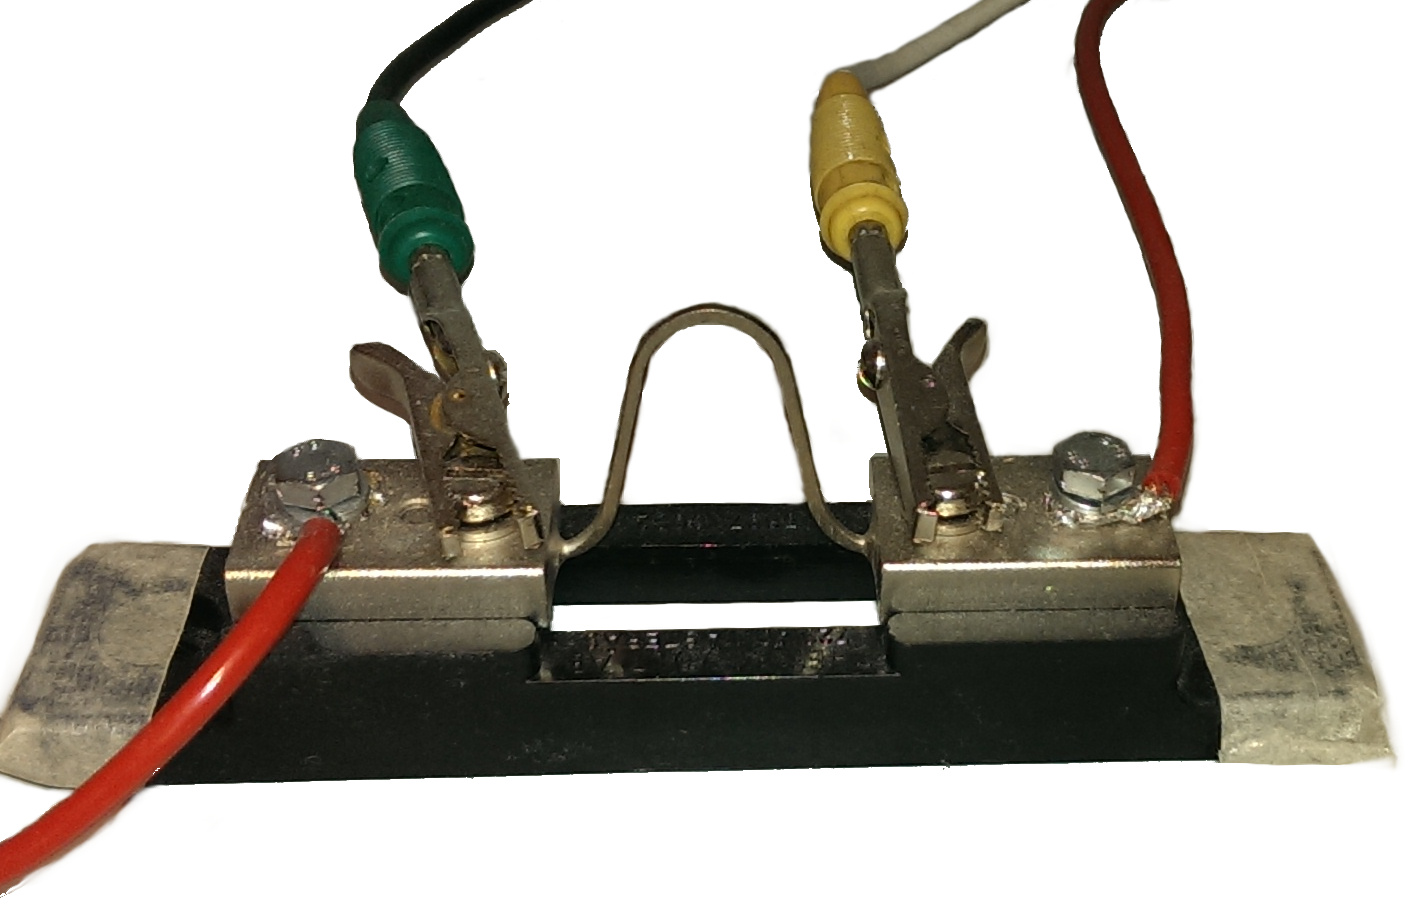
\includegraphics[width=0.8\textwidth]{figs/shunt.jpg}
    \caption{An example shunt resistor}
    \label{fig:shunt}
\end{figure}

% TODO: Where does this fit?
% The ultimate goal in this context is to estimate power consumption and energy
% efficiency of new hardware, the first step is to measure different more or less
% power consuming events on real hardware that is similar to the one simulated.


\section{Hardware Platform}

The ODROID-X2 developer platform \cite{hardkernelodroidx2} is used as a
reference hardware for all experiments in this thesis. An image of the platform
is shown in \autoref{fig:odroidx2}. Its core voltage is easily accessible on an
attached daughter board right beneath the heat sink, making it easy to conduct
power measurements. The board is equipped with a Samsung Exynos 4412 ``Prime'',
a modern System-on-Chip featuring four ARM Cortex-A9 CPU cores, Mali-400 GPU and
2~GB of on-chip DRAM. The Cortex-A9 is one of ARM's mid-to-high-range application
processors. It features an out-of-order dual-issue speculative RISC core, and it
is clearly designed with emphasis on energy efficiency. This processor is
primarily found in low-powered embedded devices with some performance demands,
typically smartphones and tablets.

\begin{figure}[bth]
    \centering
    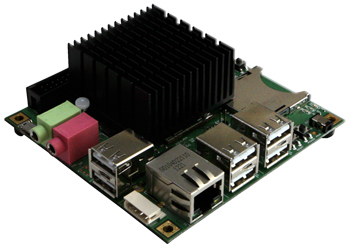
\includegraphics[width=0.7\textwidth]{figs/odroid.jpg}
    \caption{Image of the Hardkernel ODROID-X2 from the Hardkernel ODROID-X2 product page \cite{hardkernelodroidx2}}
    \label{fig:odroidx2}
\end{figure}

\begin{table}
    \centering
    \begin{tabular}{|c|c|}
        \hline
        Component      & Spesification\\
        \hline
        Manufacturer   & Hardkernel \\
        Platform       & ODROID-X2 \\
        SoC            & Samsung Exynos 4412 ``Prime'' \\
        CPU Core       & ARM Cortex-A9 \\
        Number of Cores& 4 \\
        Clock Frequency& 1.7~GHz \\
        Core Voltage   & 1.3~V \\
        L1             & Dual 32~KB \\
        L2             & 1~MB \\
        Main memory    & 2~GB LP-DDR2 880~MHz \\
        \hline
    \end{tabular}
    \caption{Hardware specifications ODROID-X2}
    \label{tab:hwspecx2}
\end{table}

As seen in \autoref{fig:a9arch} there is an out-of-order multi-issue module
right after the decode stage. This module can do speculative issue and can
schedule two arithmetic operations, in which one can be a multiply (the
processor has only one hardware multiply unit). It also features a multiplexed
lane for address operations and floating point operations (the \emph{NEON} FPU).
In this experiment, a 4-core variant of the processor was used, but 3 of the
cores was disabled to ease both the measurement and the simulation process.

\begin{figure}[bht]
    \centering
    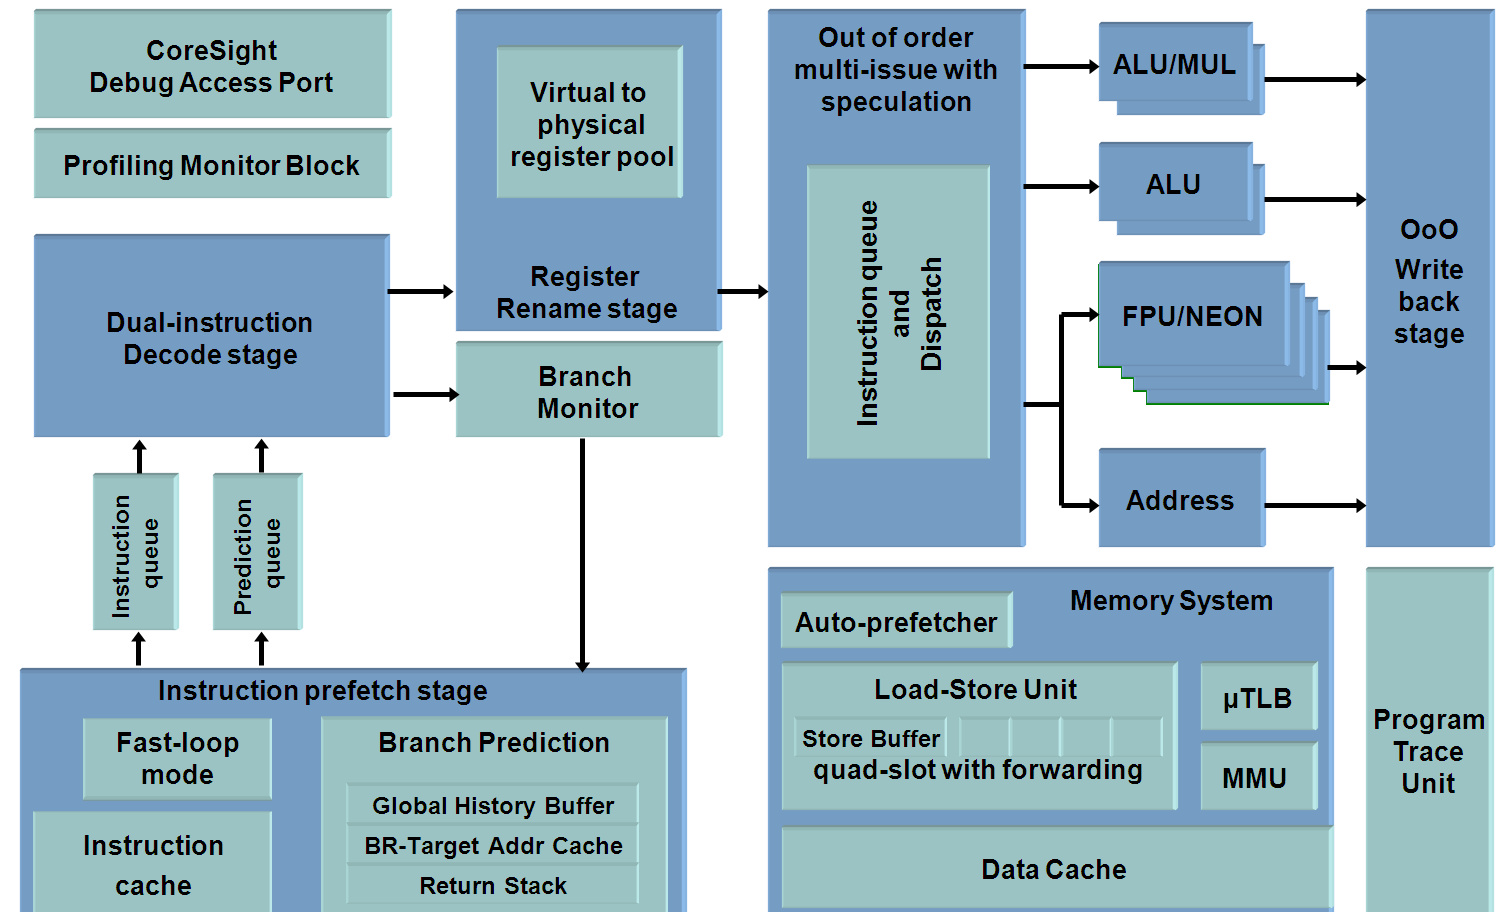
\includegraphics[width=0.8\textwidth]{figs/A9-Pipeline-hres.jpg}
    \caption{A brief overview of the Cortex A9 Pipeline, figure from the ARM Cortex-A9 Whitepaper \cite{a9whitepaper}}
    \label{fig:a9arch}
\end{figure}

To achieve good simulation correctness, a high level of architectural knowledge
is crucial. Despite that most proprietary architectures have a lot of details
that remain undisclosed to the public, much information is still available.
Different sources have been used to find properties needed by the simulator,
some details regarding the OoO cores can be read about in
\cite{blem2013detailed}.

\section{Hardware Simulators}

As computer architecture development meets more challenging demands, a versatile
set of software tools have been developed to help the designers. In this set of
tools lies a set of computer architecture simulators meant to evaluate
processors at the architectural level. The simulators often provides the ability
to write hardware in a language more abstract than HDL-languages, provides the
ability to run compiled binaries, and provides detailed trace logs and
performance data. The benefits of architectural simulators are many, but it is
important to find one that fits the demands given by the problem.

\subsection{A Brief Comparison}
\label{subsec:simulators}
There are numerous computer architecture simulators available to the public,
both commercial, free and open source alternatives exists. To support our power
estimation tool, a simulator frontend must provide a good picture of events
that occur in a hardware implementation of the architecture. The hardware
platform used for reference in this thesis is an out-of-order ARM Cortex-A9
based core fitted with memory and and peripherals in a von Neumann architectural
scheme. The out-of-order property significantly increases the level of
complexity which the simulator must handle.

\begin{description}
\item[Sniper] \hfill\\
    Sniper is a high-speed, multicore, multi-threaded and cycle-accurate
    computer architecture simulator \cite{sniperwebpage,carlson2013ssomta}. It
    already integrates with McPAT and it is open source. Sniper does only work
    x86, and is thus not applicable for simulation of ARM-based architectures.

\item[SimpleScalar] \hfill\\
    SimpleScalar is a popular commercial architectural simulator that comes with
    a free academic license providing full source code. SimpleScalar supports
    the ARM instruction set amongst many others, and looks like a decent
    simulator for advanced out-of-order core simulation. SimpleScalar is also
    the simulator used by the Wattch-project \cite{brooks2000wattch}. However,
    the SimpleScalar web page seems to be last updated in 2004 and all mailing
    list archives are gone at the time of writing. The source code for
    SimpleScalar v3 is still available, but has only been patched once since
    2003.

\item[QEMU]\hfill\\
    QEMU is a generic and open machine emulator which enables near real-time
    performance on architectures like ARM, even on x86 host machines. However,
    QEMU is a machine emulator rather than an architectural simulator, thus
    despite its great performance of running ARM-binaries, it will not produce
    CPU and memory event trace logs, and is not suitable for this project.

\item[gem5]\hfill\\
    gem5 is a merger between the M5 simulator \cite{binkert2006m5} and the GEMS
    simulator project \cite{GEMS}. gem5 provides ARM-support with out-of-order
    execution out of the box, and provide great cycle-accurate trace logs which
    are appropriate for this project \cite{gem5simulator}. Its core is written
    in C++ and has a highly modular interface that allows users to specify
    simulator target through simple Python scripts. Many of the maintainers are
    employees of ARM Corp., and the activity on the mailing lists suggests high
    project activity \cite{gem5dev}.
\end{description}

Provided this comparison of simulators, and given the fact that NTNU has a tradition
for using M5 and gem5 in earlier research projects and subjects, gem5 is the natural
winner for the choise of an architectural simulator.


\subsection{The gem5 Simulator}

The gem5 project \cite{gem5} merges the best features of M5 \cite{binkert2006m5}
and GEMS \cite{GEMS} and includes a wide range of CPU and memory models
\cite{gem5hipeac}. The simulator has two main execution modes; \textit{Syscall
Emulation} (SE) or \textit{Full System} (FS). In SE mode, the simulator traps
system calls in the binary and emulates them, often by passing them to the host
operating system. In FS mode, the simulator can load an operating system binary
and run application within the OS. The latter mode is well suited when the OS in
its entirety must be simulated. gem5 supports many architectures; it can run
binaries compiled for ALPHA, SPARC, MIPS, ARM, x86 and POWER architectures.

During simulation, gem5 keeps track of hundreds of events related to the CPU
core and memory system. In-detail statistics, similar to performance counters on
real hardware, are then dumped for subsequent inspection. gem5 is also able to
output a trace log while it runs, originally intended for debugging of gem5.A
trace log contains user-selected events that happens within the simulated
hardware. These trace logs grow quickly in size, easily 10s of gigabytes, but
provides useful insights of the simulated execution. In particular, they describes
CPU activity down to the microarchitecture level and outputs simulated processor
activity.


\section{Parameter Optimization}


\subsection{Genetic Algorithms}

\section{SHMAC}

SHMAC is a hardware prototype of a Single-ISA Heterogeneous MAny-core Computer
\cite{shmacsliedes, shmacwebpage, Rusten567042}. It is an ongoing research
project within the Energy Efficient Computing Systems (EECS) research area at
the Department of Computer and Information Science at NTNU. The SHMAC project is
driven by the \textit{dark silicon effect}; as transistors become smaller, only
parts of a chip can be powered simulataneously \cite{esmaeilzadeh2011dark}.
SHMAC implements two main strategies to mitigate the dark silicon effect,
heterogeneity and specialization.

\begin{figure}
    \centering
    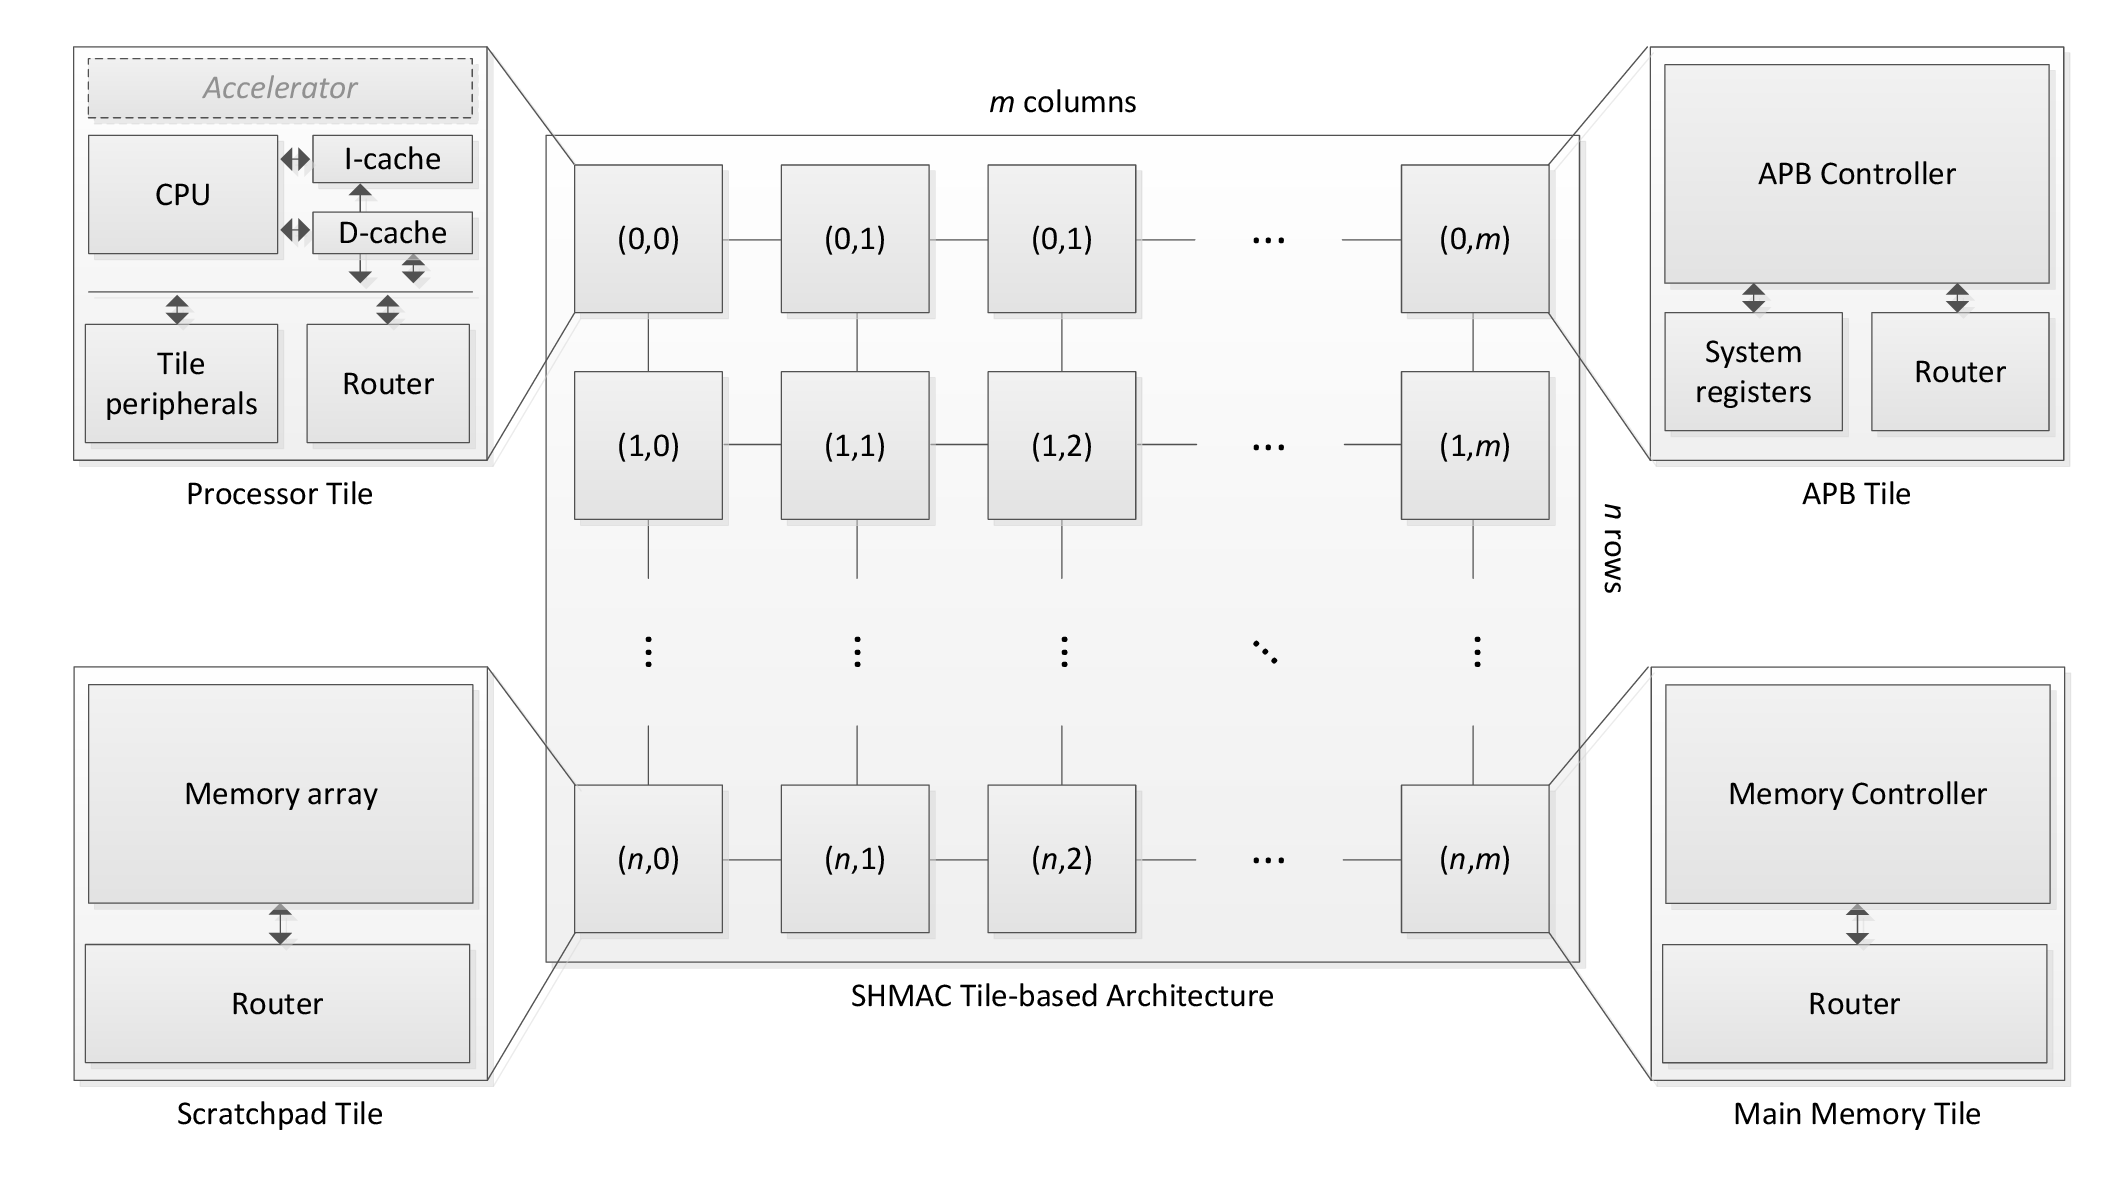
\includegraphics[width=1.0\textwidth]{figs/shmac-high-level2.png}
    \caption{}
    \label{fig:shmac}
\end{figure}

The SHMAC architecture is tile-based. Processing elements are laid out in a
rectangular grid with connections to their nearest neighbor, as depicted in
\autoref{fig:shmac}. A router protocol present in all SHMAC tiles handles
communication and data flow between tiles.  The great deal about SHMAC is that
different kinds of specialized tiles/accelerators can be composed as desired, to
form a computer tailored to the application.


\chapter{Building PET}
PET is a Power Estimation Tool that provides guided information about power
usage for new architectures, and represents a major piece of our problem
solution. The following chapters will describe how it works along with it's
strengths and weaknesses.

\section{What is PET?}

\begin{figure}
    \includegraphics[width=0.9\textwidth]{figs/pet-workflow-gv.pdf}
    \caption{Workflow using PET}
    \label{fig:workflow}
\end{figure}

PET is built by measuring real hardware with great detail, capturing discrete
events and assigning each event a certain energy cost. As depicted in
\autoref{fig:workflow}, when selected events have been weighted, one can run the
test program through a simulator set up to act as the new hardware. The simulator
will generate a tracelog containing the weighted events, and PET can then apply
the numbers. From this workflow, PET can produce a data set containing power
consumption distributed over the simulation lifetime. As noted, the new hardware
will be weighted equally of a chosen existing hardware, so so this method
requires a certain similarity beteen the new and the old hardware. In general,
all traditional architectures contains equal principles of function, and is thus
mappable to each other, but accuracy will of course differ as hardware differs
in design, applied voltage, clock speed and process technology.

When estimating power usage for new architectures, it is hard to pick events and
assign a cost to it. We will have to assume that the new architecture is
comparable to an old architecture, so that we can use the old power estimation
numbers to guide a new estimate. For instance, one can experiment with a
larger L2 cache to see how it affects energy usage (and performance). The
additional energy a larger L2 cache uses can be found from existing
implementations.

\section{Methodology}

While computer architecture simulators have been around for quite some time,
energy estimation techniques is a more recent necessity. Song et. al
\cite{song2012instruction} identifies three major approaches to processor power
modelling used in the past, and introduces an instruction-based energy
estimation model that can be used for energy simulation at high speed. Their
proposed method is expressed through the following equation and includes the
desired features of past energy models.

\[
    P_{core}(t) = \frac{E_{unit} \cdot A_{datapath} \cdot w(t) +
    E_{static}}{T_{sampling}}
\]

This method depends on two things. First, one must know sufficient details of
the processor to identify datapath components in order to form the
$A_{datapath}$ matrix. Secondly, the energy unit vector $E_{unit}$ requires
circuit-level knowledge of the target processor. The former information can
often be found by reverse engineering and benchmarking, however, the latter is
rarely available for commercial processors. When building the model for PET, we
simplify the model from \cite{song2012instruction} by combining $A_{datapath}$
and $E_{unit}$ to form a vector of weights that directly corresponds to the cost
of an event. We can then model energy by the following formula.

\[
    P_{core}(t) = \frac{C \cdot w(t) + E_{static}}{T_{sampling}}
\]

Here, C represents the global cost vector -- a matrix enumerating the cost
for all event types. Please note that it is global and do not depend on time.

The choice of events/workload metrics is an important part of our method. We
account for two types of events; CPU instruction events and memory activity
events.

A major design choice made on how PET should be designed was decide whether it
should be a standalone program or incorporated into an existing simulator.
There already exists a lot of computer architecture simulators, all with
strengths and weaknesses. Often, simulators only supports a small set of
architectures, memory systems and CPU models, and they only excel in simulating
one specific combination.

\subsection{A brief comparison of simulators}
\label{subsec:design_choices}
There are quite few active and open projects trying to estimate power
consumption of unimplemented platforms. Since the public available information
regarding such approches are sparse, this thesis will try to reason some about
the design choices on its own.


\begin{table}
    \begin{tabular}{l|c|c|c|c}
        Name    &   Simulated Architectures & Active & License & Notes \\
        \hline
        gem5    &   Alpha, & Yes & BSD/MIT/LGPL & in-house experience \\
        MARSSx86&   X86-64 & Yes & GPL-v2       &                     \\

    \end{tabular}
\end{table}

\subsection{Power Consuming Events}
It is desirable to estimate energy consumption on literally all types of
compututing systems, ranging from large-size clusters to embedded systems. To
provide this flexibility it was decided to write the tool as simulator agnostic
as possible, tracking \emph{simulator events} rather than executed instructions.
A simulator event is defined as a unit of work that uses a specified amount of
energy, and increases modelled energy consumption to the simulated time. We
defined a set of simulator events that PET should consider. The selected events
are briefly described in \autoref{tbl:events}.

\begin{table}[ht]
    \centering
    \begin{minipage}[b]{\linewidth}
        \centering
        \begin{tabular}{|l|l|}
            \hline
            IntAlu    & Integer basic ALU operation\\
            \hline
            IntMult    & Integer multiply ALU operation \\
            \hline
            MemRead    & Memory Read issued, triggers LS-unit \\
            \hline
            MemWrite    & Memory Write issued, triggeres LS-unit \\
            \hline
            SimdFloatMisc     & NEON-unit activated \\
            \hline
        \end{tabular}
%        \subcaption{CPU Core Events}
    \end{minipage}

    \begin{minipage}[b]{\linewidth}
        \centering
        \begin{tabular}{|l|l|}
            \hline
            L1IR    & L1 instruction cache, read \\
            \hline
            L1IW    & L1 instruction cache, write \\
            \hline
            L1DR    & L1 data cache, read \\
            \hline
            L1DW    & L1 data cache, write \\
            \hline
            L2R     & L2 cache, read \\
            \hline
            L2W     & L2 cache, write \\
            \hline
            PhysR   & Main memory, read \\
            \hline
            PhysW   & Main memory, write \\
            \hline
        \end{tabular}
%        \subcaption{Memory Events}
    \end{minipage}
    \caption{Power Consuming Events}
    \label{tbl:events}
\end{table}


gem5 was used as a basis for development and the only simulation front-end
implemented.




- ARM support (Sniper has not)

QEMU -- feil abstraksjonsnivå/formål
McPat - multicore, power AND AREA???? Optimizer
CACTI - cache power estimation
gem5 is flexible because
- it is easy to add new processor architectures
- memory system
=> in-house experience

LLVM traces?


\section{Architecture}

Modern computer science emphasize parallelism as a highly important property in
order to achieve speed on multicore processors. As the size of the log files
which PET has to parse can easily be 10s of gigabytes large, PET has to be
designed with performance in mind. This means that PET must be lightweight and
parallel in order to be fast, while it must maintain correctness and be easy to
use.

Due to memory constraints on commonly available computers, it is not feasible to
read the entire log file into memory and then start parsing. It would also make
the reading step a serial part of the program, which hinders parallelism. It
will also be a bad idea to read one line, parse it, weight it and apply it to
the grand total, as it would be an entirely serial process.

\subsection{Overview}

\begin{figure}[ht]
    \includegraphics[width=0.9\textwidth]{figs/pet-pipeline-gv.pdf}
    \caption{How PET works}
    \label{fig:pipeline}
\end{figure}

In order to maintain good speed while still keeping the PET source code
readable, we have looked at different ways of chewing through large data sets.
The final implementation of PET follows a scheme borrowing ideas from the
producer-consumer patterb as explained by Gamma et. al. in \cite{designpatterns}
and the MapReduce algorithm \cite{dean2008mapreduce}. As depicted in
\autoref{fig:pipeline}, this scheme makes it rather easy to let a producer read
the lines from the log file into ring buffers (produce) and let multiple
consumers pick from each their ring buffer (consume). Each consumer parses the log
lines they pick, and apply the weight of each read event to each their result
vector (map). When all lines are read and parsed, the results vectors are
merged, and idle-task power and static power consumption is added (reduce). This
combination of algorithms allows PET to take advantage of as many cores as
possible, limted only by how fast the producer can read the log files. Finally,
a human readable output is produces, either as a gnuplot line graph or as
formatted or plain text output.

The next subsections will describe in detail the most imporatant parts of the
workflow. For further understanding of the program flow, a call graph extracted
from the entire source code can be found in \autoref{fig:callgraph}.

\begin{figure}
    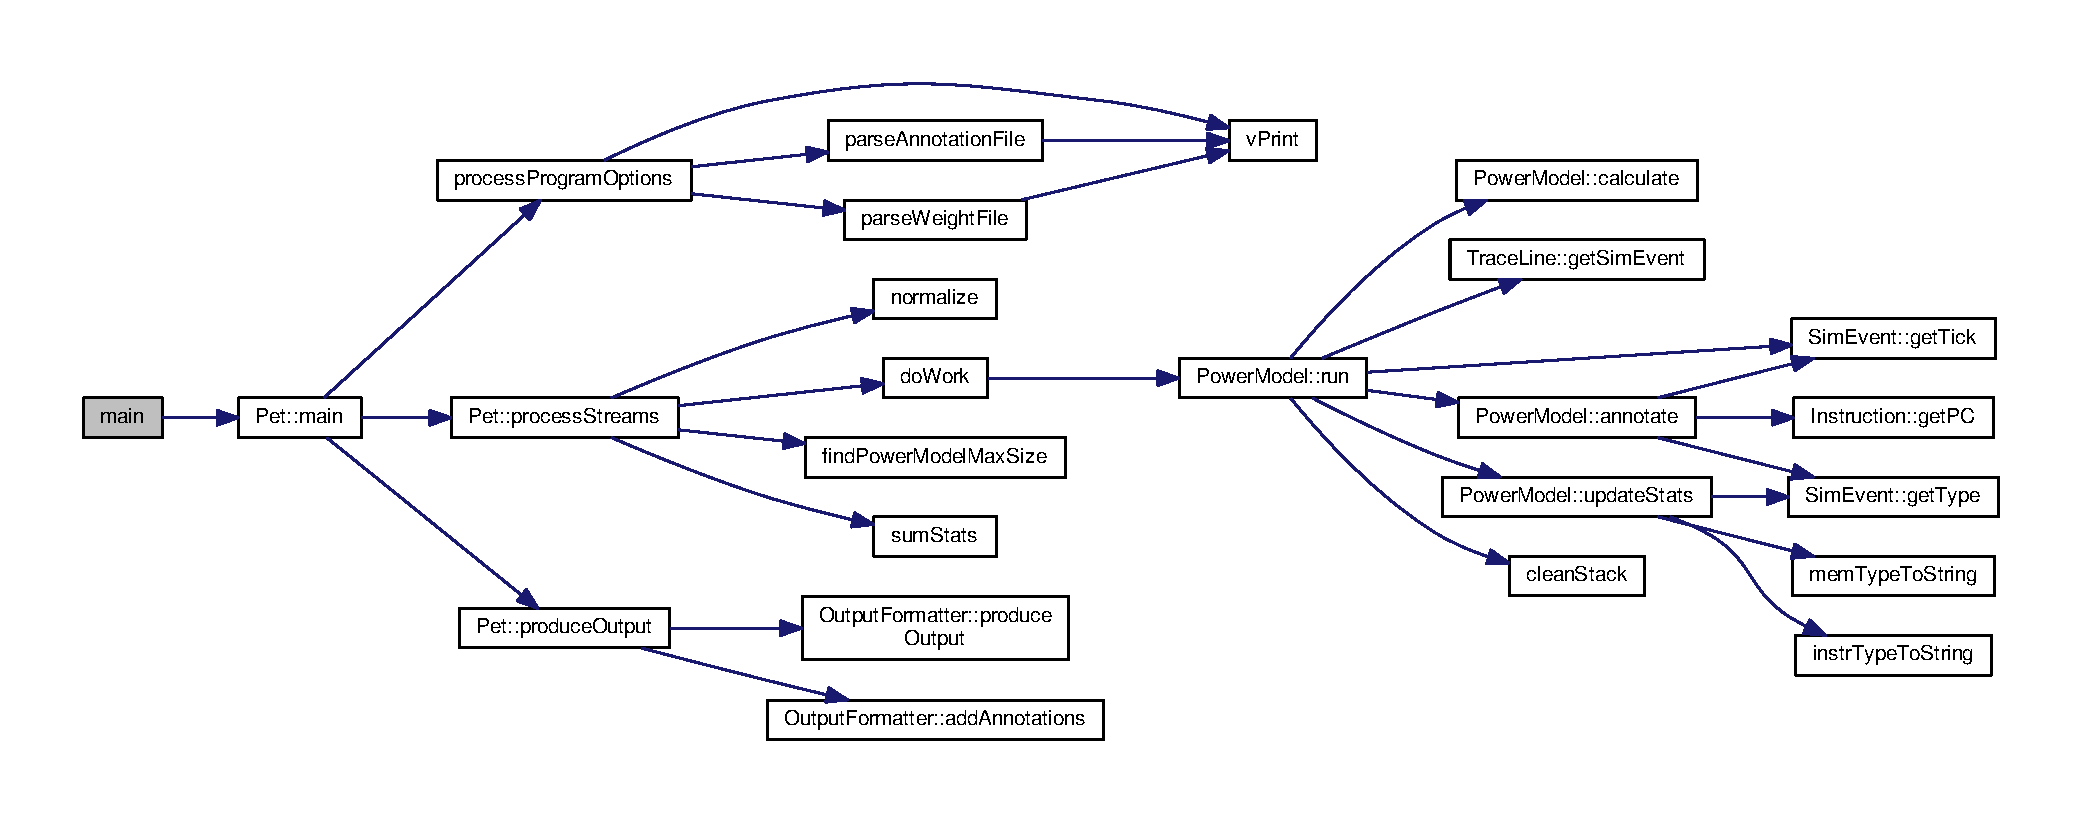
\includegraphics[width=\textwidth]{figs/maincallgraph.pdf}
    \caption{Call graph}
    \label{fig:callgraph}
\end{figure}



\subsection{Argument Parsing and Program Options}

As any other non-trivial programs, PET has to adapt to input options given from
the command line or from a settings-file. PET makes extensive use of the
\texttt{Boost}-library \cite{boostwebpage} and utilize
\texttt{Boost::Program\_options} for parsing the command line. Making use of
\texttt{Boost} for common tasks all over the program made the development cycle
less cumbersome and more rapid. \texttt{Boost::Program\_options} allows easy
extraction of program options, both with long (\texttt{\textemdash \textemdash
option=\emph{value}}) and short (\texttt{\textemdash o~\emph{value}})option
style.


\subsection{Reading Trace Logs}

When arguments are parsed and a trace log has been specified, either by path or
as \texttt{stdin}, a single thread is kicked off reading each line of the log
file into a C++ string container. This happens in the
\texttt{Pet::processStreams} method seen in \autoref{fig:callgraph}. The string
container is then inserted into one of many circular buffers. The circular
buffers are implemented with \texttt{boost::lockfree::spsc\_queue}, a lock free
single producer, single consumer queue. The property of beeing lock free is
explained by Tim Blechmann and the boost-community in \cite{boostlockfree} as
follows: "data structures are \emph{lock-free}, if some concurrent operations
are guaranteed to be finished in a finite number of steps. While it is in theory
possible that some operations never make any progress, it is very unlikely to
happen in practical applications". In PET, this queue has a fixed size of 8192,
but dynamic size is also available in the library implementation.

Which buffer the string is inserted into is determined by a simple circular
algorithm; the next ring buffer is selected when current one is full. When the
buffers are small enough to be filled fast enough to let all workers do work,
this method creates a lot less locking than using a single ring buffer shared by
all worker threads. The number of threads and the size of the ring buffers are
tightly coupled with how fast the host computer is able to feed PET with the log
files.

It is our experience that reading the log file is not the bottle neck, and it is
easy to feed at least 8 cores when the log file is hosted on a reasonable fast
drive. A simple benchmarking done with PET running on a system consisting of an
Intel Core i7 4820, 32GB DDR3 SDRAM and keeping the log files on a fake-RAID
Level-0 consisting of two Western Digital Caviar Black 750GB disks shows this.
PET running with 8 threads on this particular system is consuming the log files
with a rate of 133MB/s regardless of where the log files resides in RAM or on
disk. The benchmark used a log file of 5458MB and was run in 40.871 seconds.

\subsection{String to Event Mapping and Power Accumulation}

String parsing and mapping resembles the most compute-intensive parts of PET.
These parts of the program is kicked off as thread starting the
\texttt{doWork}-function, as the thread library cannot start running in methods
of instanceiated objects. As displayed in the callgraph in
\autoref{fig:callgraph}, this function simply starts the
\texttt{PowerModel::run}-method on its input, which an instance of the
PowerModel-class.

As the producer fills the ring buffers for each of the workers, the workers pick
strings from their pool. The strings are popped from the ring buffer, thus
making space for new elements right away. Each string is parsed by the TraceLine
class, which looks for patterns in the strings containing known event types.
When connecting PET with gem5, the trace logs as previously seen
\autoref{lst:trace} contains an event type designation in the second :-separated
column. The TraceLine class extracts this part using a very simple method to
make this part go fast, outline of this method is listed in
\autoref{alg:extract}.

\begin{algorithm}
    \begin{lstlisting}[style=algo,language=python]
function extractEventType( line ):
    start = line.find(":") + 1
    end = line.find(":", start)

    while (line[start] == ' ')
        start = from + 1
    while (line[end-1] == ' ')
        end = to - 1

    return line.substring(start, end)
    \end{lstlisting}
    \caption{Event Type Extraction}
    \label{alg:extract}
\end{algorithm}

In the real program, some more error handling is present, and the event types
are instanceiated as objects of their parent type (Instruction- or
Memory-event). The right parameters are further found from progressive string
parsing. If the event is not recognized, an "empty" object of type UnknownEvent
is returned, this type always has zero weight. Each event object is able to
figure out its own weight as written in the \emph{weights}-file. After the
event has been parsed, its weight is added to the power model at the right
time step.

In order to reduce the time used for disposal of the string objects
after they are parsed, they are places in a static-size array. When
this array is full, or the ring buffer is empty, the worker deletes
all the strings in a chunk. This methods keeps the memory footprint
low while not calling \texttt{free()} at a continuous rate. The \texttt{free()}
function is not considered very slow, but from the reference implementation
shown in \cite{kernighan1988c}, it does contain enough pointer
arithmetics to make a difference in a tight loop.

\subsection{Data Reduction}

When all lines from the trace log are consumed by the workers, the threads are
joined and their data is returned as standard C++-vectors. These result vectors
are further wrapped in yet another standard C++-vector. The inner vectors is
then looped over together, and the value from the current data point in each
vector is added together and put in a result vector. This accumulation happens
as the last part of \texttt{Pet::processStreams} as seen in
\autoref{fig:callgraph}. After a single point has been accumulated from the
vectors, idle time is calculated from how many events that was recorded during
the data point. This is done more simplistic than accurate using
\autoref{eq:idle}. $numEvents$ is the number of events recorded in each vector
at each measure point, and each event is pinned to the cycle where it
originated.

\begin{equation}
    totalEvents = \sum_{n=1}^{N} numEvents_n
\end{equation}
\begin{equation}
    idleEvents = \frac{ticksInDatapoint}{ticksInCycle}- totalEvents
\label{eq:idle}
\end{equation}

It should be noted that even though this method might work well in a
single-cycle in-order CPU, the out-of-order nature of the Cortex-A9 makes it
hard to tell how much idle time actually exists. E.g. A single cycle may fill
the pipeline with four events, then idle the three next cycles; this would be
calculated as no idle time. When the approximate numbers of \texttt{idleEvents} have been
estimated, that number is multiplied by the \emph{Idle}-weight and added to the
sum in the result vector. Finally, the entire vector is normalized according to
bucket size and then static current drain is applied.


\subsection{Output Production and Annotations}

After the result vector has been completely accumulated, annotation
is added to a new result vector in the same manner as the data reduction.
With the new, merged annotation map containing all last matches between
a symbol and the program counter within each measure point, this map
is feed to the \texttt{OutputProducer}-object as seen in \autoref{fig:callgraph}.
The \texttt{OutputProducer}-object is responsible for generating output as defined
by the input arguments. Its options have already been described in \autoref{sec:output},
and its implementation is a simple nested if-else-clause that calls internal functions for
each output type. The graphical output is produced using a wrapper around GNUPlot, while
the textual outputs are created by \texttt{printf}-statements.


\subsection{Unit Tests}

All internal string parsing are verified by unit tests. The unit tests
are written with help from the Boost Test Library Unit Test Framework \cite{boostunittest}.

The test library generates a new binary with the same program content, except the
main function, thus the program flow, is different. The test binary will
run through the listed functions with a certain input, and if the output is unexpected,
the test binary will print to the console an error message containing a description of what
went wrong. This approach helps refactoring and correctness in general, such that
the focus can be kept on the program surroundings.


\section{Input}
New hardware architectures are not easily analysed without physical
implementation, but often we are able to simulate its behaviour to acceptable
accuracy, and thus we are able to test different implementations with low cost.
These simulation runs can often be set up to produces trace logs which contains
a user controlled amount of detail. PET can use these trace logs and scan them
for predefined events, each affecting the power consumption of the simulated
hardware. Different simulators have different trace log formats and different
trace abilities. We have chosen gem5 as our target simulator as it is easy to
configure, and trace is well implemented. As mentioned in
\autoref{subsec:design_choises} other options are available, but the support for
easily configurable CPU- and memory system along with the pre-implemented ARM
processors and in-department hands-on experience with this simulator made gem5
the most logical choise.

\subsection{gem5 trace logs}
When run with \texttt{--debug-flags=Bus,Cache,MemoryAccess,Exec} gem5 will output trace files look like
the text displayed in \autoref{lst:trace}.

\begin{lstlisting}[basicstyle=\tiny,caption={gem5 trace log},label={lst:trace},escapeinside={@}{@},float]
@\label{line:physmem}@3021: system.physmem: Write of size 8 on address 0x82fe0 data 0xe1a0f00eee1d0f70
@\label{line:icache}@3021: system.cpu.icache: access for ReadReq address 9c0 size 64
@\label{line:cachemiss}@3021: system.cpu.icache: ReadReq (ifetch) 9c0 miss-
...
@\label{line:cacheupdate}@3432: system.cpu.dcache: Block addr 81f0 moving from state 0 to state:7 valid: 1
3432: system.cpu.dcache: Leaving recvTimingResp with ReadResp for address 81f00
3432: system.tol2bus.respLayer1: The bus is now busy from tick 234320 to 236376
@\label{line:memread}@1642: system.cpu T0 : 0x89d4.0 : ldr   r1, [sp] #4     : MemRead :  D=0x00000000
@\label{line:intalu}@1642: system.cpu T0 : 0x89d4.1 : addi_uop   sp, sp, #4 : IntAlu :  D=0x00000000b
1701: system.cpu T0 : 0x89d8   : mov   r2, sp          : IntAlu :  D=0x00000000b
1701: system.cpu T0 : 0x89dc.0 : str   r2, [sp, #-4]!  : MemWrite :  D=0x0000000
1760: system.cpu T0 : 0x89dc.1 : subi_uop   sp, sp, #4 : IntAlu :  D=0x00000000b
1760: system.cpu T0 : 0x89e0.0 : str   r0, [sp, #-4]!  : MemWrite :  D=0x0000000
4000: system.membus: recvTimingResp: src system.membus.master[0] ReadResp 0x1640
4000: system.l2: Handling response to ReadResp for address 1640
4000: system.l2: Block for addr 1640 being updated in Cache
\end{lstlisting}

Each line in \autoref{lst:trace} represents an event that happens in the
simulated hardware.  \autoref{line:physmem} tells that a write access to
physical memory has happened. \autoref{line:icache} is the event of instruction
cache access, while \autoref{line:cachemiss} shows that this request failed.
During this simulation, there is also events like \autoref{line:cacheupdate}
which represents that the data cache updates some content. The discrete
instructions running through the CPU is also logged, eg. \autoref{line:memread}
shows a load-instruction and \autoref{line:intalu} shows an
addition-instruction.

As discrete events are picked out from the trace logs, PET accumulates power
consumption in equally sized timeslots, called buckets. Each bucket has a
parameter controlled size in terms of simulator ticks. Often it is more
practical to specify the number of buckets in the output rather then specifying
the number of simulator ticks in each bucket. Because of this, PET is able to
estimate the bucket size by peeking at the tick at the last line of the trace
file. It has been shown that the trace file is not nessesary in tick order,
but it will commonly be at approximatly the last tick at the last line. The
bucket size estimation algorithm is shown in \autoref{alg:bucket_size}.

\begin{algorithm}
    \caption{Bucket Size Detection Algorithm}
    \label{alg:bucket_size}
    \begin{algorithmic}
        \Function{numTicks}{$traceFile$}

        \State $eofPos \gets \Call{getSize}{traceFile}$
        \State $\Call{seek}{traceFile, eofPos - 3}$
        \State
        \State $char \gets \Call{getChar}{traceFile}$
        \While{$char \ne newline$}
            \State $\Call{seek}{traceFile, -1}$
        \EndWhile
        \State $line \gets \Call{getLine}{traceFile}$
        \State $simulatorEvent \gets \Call{parseLine}{line}$
        \State \Return $\Call{getTick}{simulatorEvent}$
        \EndFunction
    \end{algorithmic}
    \begin{lstlisting}[language=Python]
function numTicks( traceFile ):
    # Find file size
    eof_pos = traceFile.getSize()

    # Seek almost to end, avoid last newline
    traceFile.seek( eof_pos - 3 )

    # Trace from back of file to second last newline
    while not traceFile.currentChar is '\n':
        traceFile.seek_backwards

    # File stream position is now at beginning of last line
    # Parse this line
    simulatorEvent = parseLine( traceFile.getLine() )

    # Return the tick of the retreived event
    return simulatorEvent.getTick()
    \end{lstlisting}
\end{algorithm}

\autoref{lst:trace} also shows that the events in the trace log is not nessesary in their
correct order, thus PET has to be able to add power consumption to the entire timeline at all
time. This means that we are unable to produce continous output, but have to store the
results in memory and dump them when the entire input is parsed.


\subsection{PET weight files}
Equally important as finding the correct events is assigning each event the
correct amount of power consumption. As each event will count differently
depending on the architecture, PET will read a weight file along with the gem5
trace log. A sample weight file is listed out in \autoref{lst:weights_example}.
As the timeslots are specified in simulator ticks instead of CPU cycles,
the values have been chosen to match a 2GHz processor, which then means
one CPU cycle pr. 500 simulator ticks using standard gem5 simulation granularity.
If you are applying this method to a processor with a different clock speed than
2GHz, be aware that the numbers has to be scaled propotionally. This is not the
case for the static power drain, as it is simply added to each timeslot, and is
not scaled in accordence with bucket size. It is also important to understand that the weight
is applied once for each event, so events that naturally takes a number of cycles
will have a high weight which is in reality distributed over many ticks. This will
not be accurate if an expensive event is applied at the border of a bucket, but we
assume that accuracy at this level is not important enought to add complexity to PET
in order to get correct.

\lstinputlisting[caption={Weight file example},label={lst:weights_example},float,language=Python]{examples/weights.conf}

The weights displayed in \autoref{lst:weights_example} are assigned and
accumulated each time PET discovers a recognisable event in the log file. A
simplified version of this algorithm can be found in
\autoref{alg:power_accum_algo}

\begin{algorithm}
\caption{Power Accumulation Algorithm}
\label{alg:power_accum_algo}
\begin{lstlisting}[language=Python]
# map of accumulated power for each time step
map<time,power> output

# input is all trace log lines, elements in weight file and
# the determined bucket size (number of simulator ticks in
# each bucket)

function assignWeights( traceLogLines, weightMap, bucketSize )
    # run through each line
    for each line in traceLogLines:
        # extract event parameters from line
        simulatorEvent = praseLine( line )

        # get the assigned weight from weight file
        eventWeight = weightMap[simulatorEvent.getEventType()]

        # add this weight to the output map
        output[simulatorEvent.getTick()/bucketSize] += eventWeight
    return output
\end{lstlisting}
\end{algorithm}
%weightfiles
%

\subsection{Annotation files}
\label{subsec:annot}
PET has the ability to annotate it's output using a map from PC to function name. The
simulated binary itself is not an input to PET, as it would contain to much information to display nicely in
an ordinary graph. Instead, PET comes along with a tool called \texttt{scripts/annotate.sh} which takes
a binary file as input and prints out all function names in the binary file. The binary file must be compiled
with debugging symbols for this to work. The usual situation would then be to pull out those function names you want
to annotate be editing the output from this tool, and then giving this file to PET as annotation input.

An example of how this map can look like is printed in \autoref{lst:annot}. The
left column is simply the PC value where the function label points, and the
right column is the function name.
\lstinputlisting[caption={Annotation file example},label={lst:annot},float,language=Python]{examples/annot.conf}

\section{Output}
Depending on application, different output formats might come in handy. PET
supports printing plain time power dump, a somewhat more readable table to
plain, table and a gnuplot figure with time as X-axis and power drain on the
Y-axis. The output format is understood as timeslots in which the architecture
has a certain current drain, which should be multiplied with applied voltage to
get numbers on consumed energy, heat generation and so on. The numbers are
scaled as milliamperes, which of course is equal to milliwatt if voltage is
$1V$.

All output formats supports annotation of function calls. This is achieved by
giving PET a list of symbols and their corresponding program counter value. PET
will tag each power bucket with the last seen symbol within that bucket, as this
symbol is the one most likly to continue over to the next measure point. Lists
of symbols can be extracted from non-stripped binaries using the script listed
in \autoref{lst:annotscript}. This script is also included in the \texttt{scripts}-folder
of PET.

\lstinputlisting[float,label={lst:annotscript},caption={Extract symbols from binary},language=sh]{../pet/scripts/annotate.sh}

Example of the \texttt{plain} output format can be seen in
\autoref{lst:pet_output_plain}. The left column is the bucket number, while the
right column is instant current draw from the modelled architecture.

\begin{lstlisting}[float,label={lst:pet_output_plain},caption={PET Plain Output}]
0 120 memcpy
1 113 start
2 150 main
3 123 main
4 133 fun1
5 117 main
\end{lstlisting}

When reading the output directly from console, a more descriptive output format
is the \texttt{table} format. An example using this option is rendered in
\autoref{lst:pet_output_table}.

\begin{lstlisting}[float,label={lst:pet_output_table},caption={PET Table Output}]
/----------------------------------------\
|   Bucket   |   Energy   |    Symbol    |
|------------|------------|--------------|
|          0 | 120.000000 |    memcpy    |
|          1 | 113.000000 |    start     |
|          2 | 150.000000 |    main      |
|          3 | 123.000000 |    main      |
|          4 | 133.000000 |    fun1      |
|          5 | 117.000000 |    main      |
\----------------------------------------/
\end{lstlisting}

Visualization is often a good thing when inspecting old or trying to understand
new problems. As it is hard to get a good overview from huge text log files, PET
provides, as stated in \autoref{subsec:annot}. In effect, it is formatting
temporary output files and calling GNUPlot do do the hard work.

\begin{figure}
    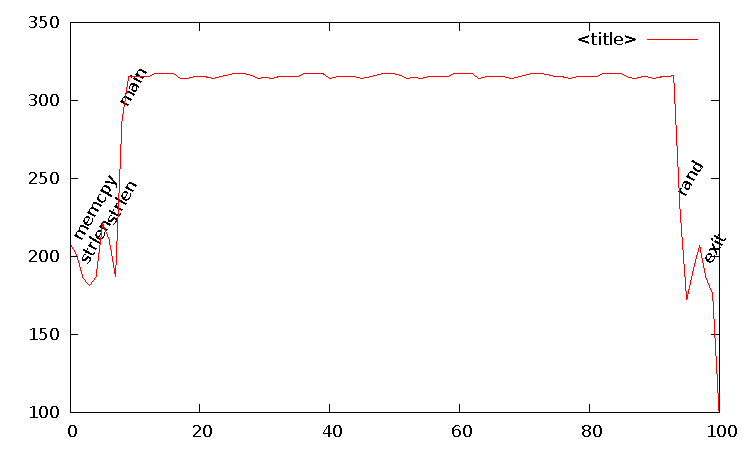
\includegraphics[width=0.9\textwidth]{figs/annot.pdf}
    \caption{PET Annotated Graphical Output}
    \label{fig:annot}
\end{figure}



usage
- input-format, input-parameter
- kjøring av gem5, flagg, se-mode
- (kryss)-kompilering av test-programmer
output
- plain, table, graph
- annotering (med eksempler på hvordan man får tak i dette)

\chapter{PET Performance Tuning}

Several factors affect the PET model accuracy. To improve accuracy, there are
many points to tune and optimize throughout the workflow. We now consider the
steps needed to adapt the use of PET on a new CPU platform. First, one must
create a CPU model using gem5's Python interface, resembling the modeled
hardware. Then, finding correct weights is formulated as a global optimization
problem.

\section{Measuring a Real World Example Processor}

The results contributed through this work relies on the existence of a method to
isolate and measure core voltage on a hardware implemented reference CPU. This
is possible due to the $V_{core}$ separation on our development kit, as
mentioned in \autoref{sec:hw}.

In \cite{rundehvatum2013exploring}, we conducted experiments to quantify the
energy cost of an instruction executing on a modern out-of-order mobile
processor. We were able to do this by completely bypassing the memory hierarchy
utilizing special hardware (\emph{fast-loop mode}) and sampling a running
average. Voltage drop over a shunt resistor such as the one shown in
\autoref{fig:shunt} was set in series with the ODROID-X2 development board is
measured, and we calculate energy used in the processor core. The results
obtained are further used to tune PET towards this architecture.

\section{Simulator Environment}

PET relies heavily on a front-end that can execute a binary on a simulator and
output $(time, event)$ tuples as a trace of execution. In this thesis, we are
using the gem5 simulator, but technically PET could be modified to support any
simulator front-end. The power profile generated by PET are derived from the
weight configuration given as input and the simulation trace, so it is important
that the simulator trace is similar to a hardware execution.

Butko et al. \cite{butko2012accuracy} reports gem5 accuracy to vary from 1.39\%
to 17.94\%, with the most accurate results coming from programs with low memory
usage. The benchmarks used represents a wide variety of scientific workloads, as
well as media applications and memory intensive synthetic benchmarks. The
program execution for their benchmarks has a high degree of instruction
diversity, so they get away with having a very simple CPU model. The real
program flow gets diluted and accurate timings are obtained simply by setting
the correct CPI value. In fact, they even use an in-order model to simulate an
out-of-order core.

We claim that the key to obtain high precision power estimates is an
architectural simulator with great accuracy. The simulator must exhibit similar
timing characteristics as the target hardware under all workloads considered,
such that the simulated execution resembles the hardware execution as much as
possible. The scheme suggested in this thesis is based on accumulation of
discrete events, each with an assigned weight according to its contribution to
the global power consumption. This means that accurate power estimation needs
these discrete events to happen, and they must happen with a realistic timing
related to their triggering cause.

Without a simulator capable of providing decent accuracy over system events,
power estimation using methods as suggested in this report will fail. We will
now explain how gem5 can be configured to improve simulator accuracy for a
particular CPU core, as well as pointing out difficulties with this approach.


\subsection{gem5 CPU configuration}
The gem5 simulator is bundled with an out-of-order ARMv7 core and serves as a
basis for the evolution of our custom core meant to model an A9 core on the
Exynos 4412. ARM cores can be configured with caches of varying sizes decided
by the implementing vendor and will have varying performance accordingly. Thus,
it is important to tune all CPU parameters so that it matches the modelled SoC.
It is not publicly known which SoC the default configuration attempts to model,
but according to the gem5 mailing list \cite{a15maillist} it is neither A9 or
A15. However, the fact that it is made for the ARMv7 instruction set and is
out-of-order makes us believe minor modifications can make it a decent model of
the Cortex-A9.

The model gem5 uses in its simulations can easily be configured using a Python
interface. We started with gem5 changeset \texttt{aaf017eaad7d} and added a new
CPU configuration file for the Exynos 4412;
\texttt{gem5/configs/common/Exynos\_4412P.py}. A few other files were edited to
accomodate the new processor definition. Please refer to
\autoref{apx:gem5files} to see all patches applied in these experiments.

As implementation details for commercial processors are hidden from the end
user, the Internet can deem helpful in the search for clues. We found many
sources of information claiming to know implementation details of the Cortex-A9,
including
\cite{blem2013detailed,butko2012accuracy,armtech,exynoswiki,odroidwiki,geekland,7cpu,armcortexa9specs}.

Combining this information helps us build a gem5 model for the Exynos SoC, but
it is still not trivial.  We found the simulator to perform different from the
physical hardware, even though the system parameters are set equal. We claim
that this is due to the abstraction the simulator provides us; the simulator is
not a complete model of the hardware. Gibson et. al. \cite[gibson2000flash] have
done a similar experiment using different simulators and concluded that bugs and
ommisions in system simulators may make performance tuning very difficult.

To improve our results, we adjust the model specification such that it
\textit{performs} similar to the hardware, i.e.  programs execute in about the
same number of clock cycles. Even if the processor implementation was completely
transparent, it would be hard to leverage the use of a multi-architecture
computer simulators. Features such as fast-loop mode found in certian ARM cores
must have a corresponding implementation in the simulator for complete
correctness, and it would be infeasible to include all details at that
granularity.

We scripted the simulator to run a wide variety of configurations, about $50$ in
total. We evaluated their performance by comparing simulated execution time to
execution time on real hardware. The final CPU configuration is shown in its
entirity in \autoref{gem5exynos4412p}.


\subsection{gem5 memory model}
The memory system is a very important part of a system simulator when doing performance estimations, but
in the time of writing, gem5 will not easily work with an out-of-order CPU model together with the GEMS Ruby
memory system. Lacking other methods considering our resources, the simple memory system will provide events
that PET can use to determin memory and memory bus communications. The simple memory model was tuned as stated
in \autoref{gem5simpledram}.

\section{Multi-objective Weight Optimization}

With an accurate CPU model, the weights must now be tuned to match measured
power consumption on real hardware. We formulate this as a multi-objective
optimization problem.

We start by creating a set of training workloads, essentially computer programs
designed to hold certain characteristics compiled to a native
ARMv7\footnote{ARMv7 is the instruction set supported by ARM Cortex-A9.} binary.
The design and selection of these will be elaborated in the next section. We
execute the binaries in the gem5 simulator with the CPU model from last
section to obtain a file containing \texttt{(time, event)} tuples from the
(modelled) execution, just like in \autoref{lst:trace}. The next challenge is to
assign each of these events a cost.

We attack this problem by running a multi-objective optimization algorithm. We
pick a subset of event types that is believed to impact energy consumption, as
we described in \autoref{subsec:powerevents}.

%TODO: Any kind of opt.alg. could have been used


We tested many evolutionary strategies
and were able to prototype quickly using DEAP \cite{DEAP_JMLR2012}, a Python
framework for evolutionary algorithms. In the end, we do not care how the
weights are found, as long as they match well to the hardware measurements.
Please note that any optimization algorithm could be used to find a proper set
of weights.

The genome is a set of CPU events, each mapped to an energy cost. E.g.
\texttt{\{IntAlu: 170, IntMult: 1300, MemRead: 80, MemWrite: 50, SimdFloatMisc:
1400, L1R: 230, L1W: 340, L2R: 1100, L2W: 1300, PhysR: 2600, PhysW: 2800\}} is a
valid individual in the population. To calculate the fitness of an individual,
we run PET with the genome weights on a set of workloads and compare the energy
profiles with measurements on hardware. Note that hardware measurements only
needs to be done once per workload. The evolution can now run without
supervision until a set of reasonable weights are evaluated.

\section{Choosing Workloads}
\label{sec:workloads}

When running a genetic algorithm, it is critical to lead the evolution in the
correct direction. In our case, this is done by providing a reasonable set of
workloads (i.e. ARMv7 programs) that stresses distinct modules in the processor.
For instance, a memory intensive workload will have high density of
memory-related events from the simulator, and will support the genetic algorithm
in determining cost for memory accesses. It is important for the set of
workloads that are chosen to be diverse and stress many conditions the processor
can operate in, e.g. mixes of compute intensive and memory intensive programs. A
poorly chosen set of workloads will not give a fair judgment on which genomes
that fit well. A bad workload might be too biased towards a few parameters,
neglecting the rest, or even mislead the GA into a local optimum
\cite{introtoga}. All training programs are compiled with soft-floats to keep
simulation complexity low. Another worry is that within the training set, there
will most likely exist multiple Pareto optimal solutions \cite{deb2014multi},
but only one of these can truly match the real power consumption.

We came up with the following four workloads.

\begin{description}
    \item[Pi] \hfill \\
        This test calculates Pi using Monte Carlo simulation. It includes
        floating point multiply and division. It runs for a fixed amount of
        iterations.
    \item[SHA-512] \hfill \\
        The SHA-512 algorithm is a hashing algorithm used in cryptography. It
        includes a mix of integer operations and memory usage. Implementation
        from \cite{sha2}.
    \item[Trend] \hfill \\
        This test has two parts. It starts with a tight add loop, and then
        continues with extensive memory allocation. Presumably, this will create
        a shift in energy consumption between the two stages.
    \item[SubMul] \hfill \\
        The SubMul test borrows ideas from the previous program, but instead of
        testing ALU and memory, this test compares subtract and multiply (both
        ALU).
\end{description}

We claim that the workloads used in this experiment spans the most common
instruction types while being simple enough to be simulated in gem5 on
reasonable time.


\section{Results}

\subsection{gem5 CPU model accuracy}

After modelling different configurations for gem5, accuracy as depicted in \autoref{tbl:gem5runtimeaccuracy}
was achieved. Each test was run with the command written out in \autoref{lst:gem5commandline}, with \texttt{CPU}
changed with  \texttt{exynos\_4412p}, \texttt{arm\_detailed} and \texttt{timing}.

\begin{lstlisting}[language=sh,label={lst:gem5commandline},caption={gem5 Command Line}]
$ build/ARM/gem5.opt --remote-gdb-port=0 -d m5out-time/sha2-sha2
    configs/example/se.py -c bin/sha2/sha2 --cpu-type=CPU
    --mem-type=LPDDR2_S4_800_x32 --sys-clock=440MHz
    --cpu-clock=1700MHz --num-l3caches=0 --caches --l2cache
    --l2_assoc=16 --l2_size=1MB --l1d_size=32kB
    --mem-size=2048MB --l1d_assoc=4 --l1i_assoc=4
\end{lstlisting}


% Move table to result chapter
\begin{table}
\centering
\begin{tabular}{|l|c|c|c|c|}
\hline
 & add-add & pi-pi & sha2-sha2 & trend-trend \\
\hline
Real hardware & 0.017600  & 0.013500 & 0.022600 & 0.014600 \\
gem5 modified O3    & 0.017541 & 0.013790 & 0.022819 & 0.011898 \\
gem5 original O3    & 0.008777 & 0.006708 & 0.010368 & 0.004344 \\
gem5 timing simple  & 0.035039 & 0.019564 & 0.040659 & 0.020503 \\
\hline
\end{tabular}
\caption{gem5 runtime accuracy (O3 with classic memory system)}
\label{tbl:gem5runtimeaccuracy}
\end{table}




\subsection{GA optimization}
As PET has been optimized by a genetic inspired algorithm, it is likly to perform very well on the data sets it
has been optimized for. When such training is done, a controll test is needed in order to verify that the result
is good for the general problem solved, not only the specific instances used for training.

\subsection{Training}

The training sets:
\begin{figure}
\centering
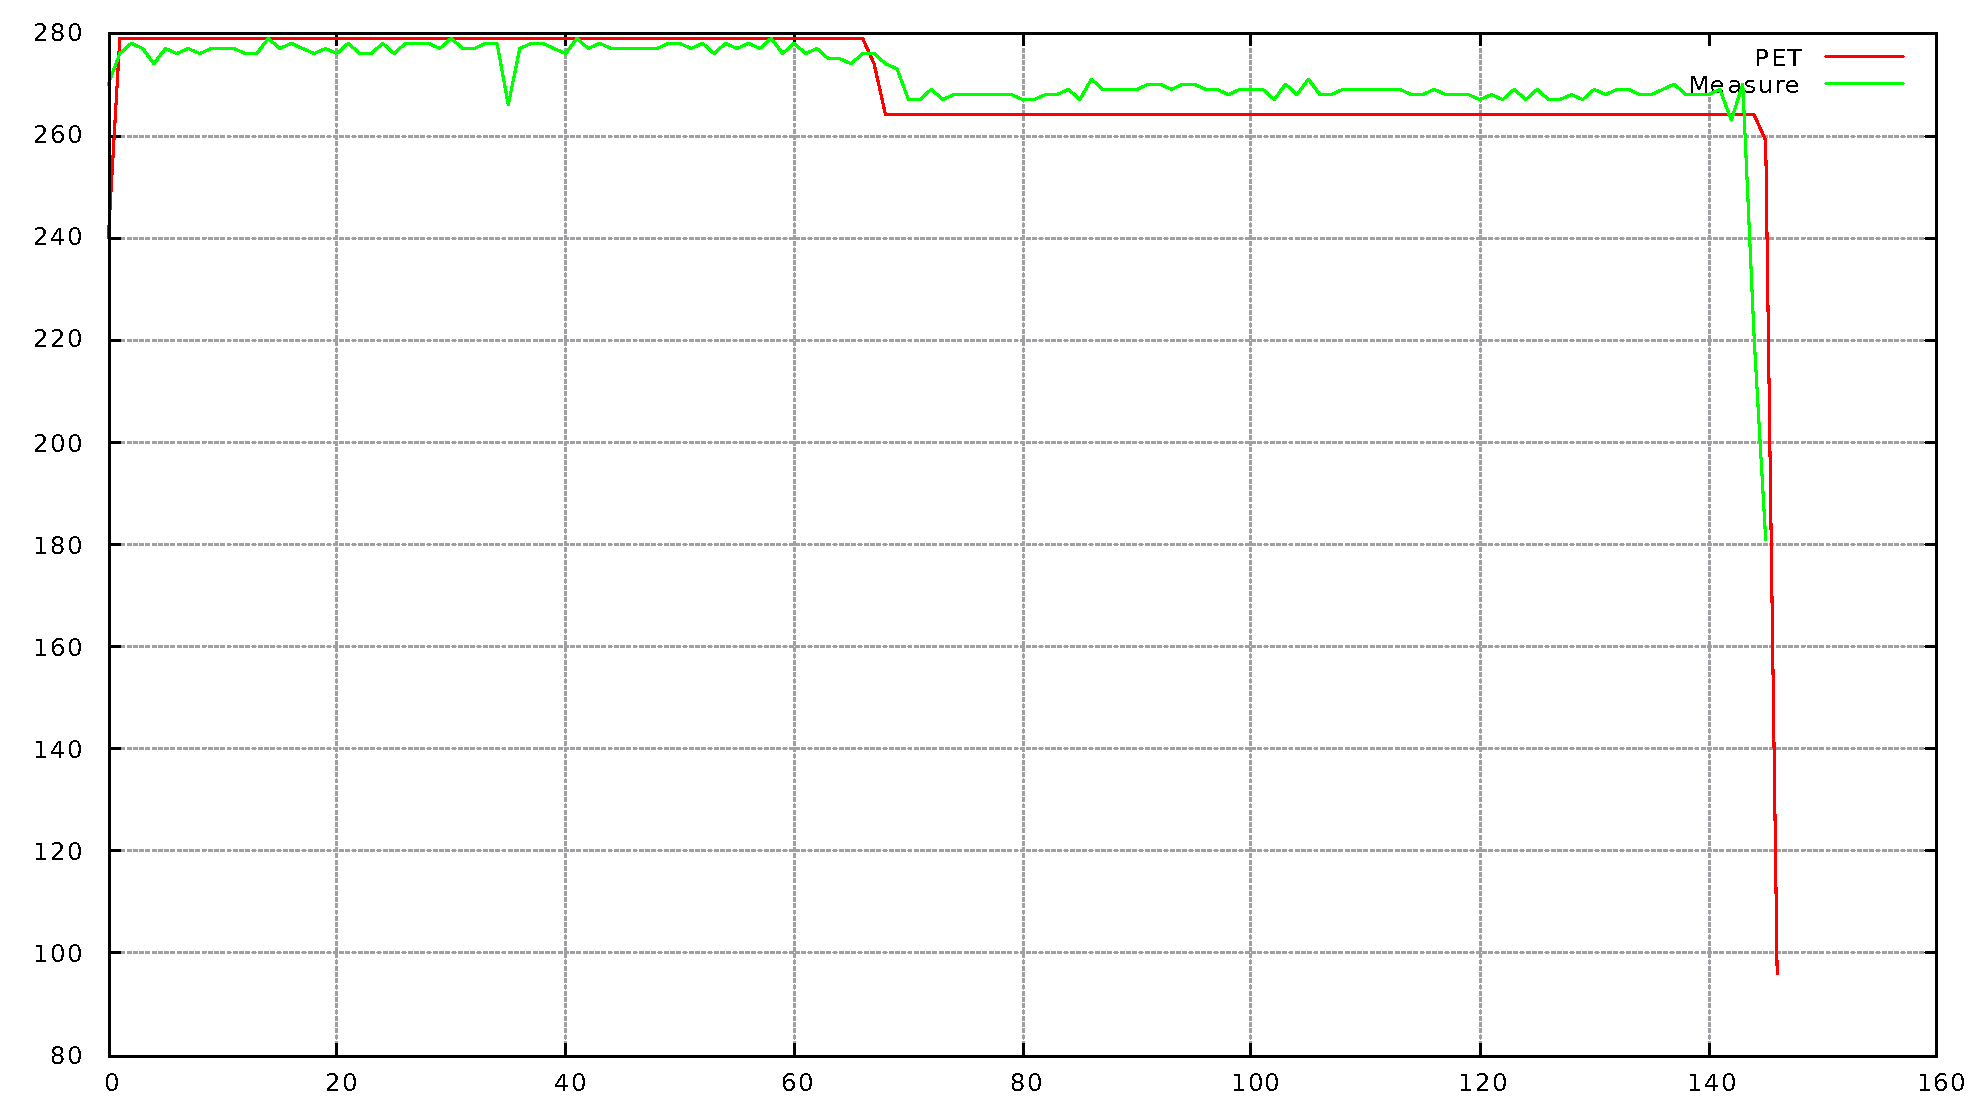
\includegraphics[width=\textwidth]{figs/trend-training.pdf}
\caption{Overlay of PET training results (red) and training data (green)}
\label{fig:trend-training}
\end{figure}




\chapter{Experiments and Results}

This chapter is about how we benchmarked PET for real world performance, referencing the fall project.

Pitfall, we only have a single architecture to test against. Consider (also not so good) solutions on how we can test other architectures?

\section{Test Environment}

PET has already proven that it is able to do the job of power estimation for the
training data. The set of workloads has been split in a training set as
presented in \autoref{sec:workloads} and a test set. This separation is
necessary in order to achieve a good result from the genetic algorithm
\cite{russellnorvig,rajer2003separation}.

The test data set consists of a short Dhrystone run and a synthetic add loop,
each representing very different use of the processor. The Dhrystone test aims
to measure overall performance of the general processor, while the add loop will
stress the ALUs leaving most of the other parts of the CPU idle. The Dhrystone
test is run for $100~000$ iterations. This is too short for a performance
benchmark, but it is long enough to measure current drain and short enough to
simulate on a simple workstation.

There are sources claiming that gem5 is very accurate
\cite{butko2012accuracy,pusdesrissources}, but these claims are done with focus
on overall performance of long-running benchmarks, not the correctness of the
architectural events. This renders a problem for PET, which needs correct
architectural events to happen in order to calculate the power profile. Yet
another important recap is that the gem5 processor model is not identical, but
merely similar to the Exynos~4412. Properties like the fast-loop mode is not
implemented in gem5 and parameters for the branch-predictor is not publicly
available. Further, this means that some discrepancy between the measurements
and PET's prediction is inevitable.

\section{Description of the Ultimate Power Estimator}
The goal of any power estimator tool would be deliver the correct answer
of how much power a certain architecture would use, but there are many
caveats making this almost impossible with our current methods.

A simple and non-complete list of things that are important with respect to power consumption,
but are very hard to get correct in a simulator are described in the following list:
    \begin{description}
    \item[Cache and memory state]
        The cache and memory systems, together with all sorts of cache prefetchers, branch predictors,
        fast-loop queues and so on will make it difficult to assure that the simulated system are in
        the exact same state as the physical system.
    \item[Interrupts]
        It is very hard to predict when interrupts will come. Interrupts mostly cause context switches,
        and thus a change in system behaviour and power drain.
    \item[CPU and system specifications not disclosed to tester]
        Unless the whole system is built in-house, there will often be certain specifications that
        are not available to the tester. PET was built against a CPU where some details where not disclosed,
        and thus it was not trivial to find the most likly details to feed to the simulator.
    \item[Real world implementation vs. simulated architecture]
        A simulated system will in most cases resemble ideas, not the exact implementation. This means
        that one can test if an idea work, but it is hardly assumed that the simulated system is exactly
        equal to any real world system.
    \end{description}
This presented list is by no means a show stopper, but tells us
that we need to focus on something that is good enough. The best power estimator that could
ever be built around a simulator would be the one that reflected the ideas of the simulated
hardware in the best way possible. Such an estimator would also give a hint about final power
consumption and its trend over a set of test programs, and would such be usable for application
specific power optimization as well as general power optimizations. PET aims to be applicable for
both these concepts.

\section{Results}

\subsection{gem5 CPU model accuracy}

After modelling different configurations for gem5, accuracy as depicted in \autoref{tbl:gem5runtimeaccuracy}
was achieved. Each test was run with the command written out in \autoref{lst:gem5commandline}, with \texttt{CPU}
changed with  \texttt{exynos\_4412p}, \texttt{arm\_detailed} and \texttt{timing}.

\begin{lstlisting}[language=sh,label={lst:gem5commandline},caption={gem5 Command Line}]
$ build/ARM/gem5.opt --remote-gdb-port=0 -d m5out-time/sha2-sha2
    configs/example/se.py -c bin/sha2/sha2 --cpu-type=CPU
    --mem-type=LPDDR2_S4_800_x32 --sys-clock=440MHz
    --cpu-clock=1700MHz --num-l3caches=0 --caches --l2cache
    --l2_assoc=16 --l2_size=1MB --l1d_size=32kB
    --mem-size=2048MB --l1d_assoc=4 --l1i_assoc=4
\end{lstlisting}


% Move table to result chapter
\begin{table}
\centering
\begin{tabular}{|l|c|c|c|c|}
\hline
 & add-add & pi-pi & sha2-sha2 & trend-trend \\
\hline
Real hardware & 0.017600  & 0.013500 & 0.022600 & 0.014600 \\
gem5 modified O3    & 0.017541 & 0.013790 & 0.022819 & 0.011898 \\
gem5 original O3    & 0.008777 & 0.006708 & 0.010368 & 0.004344 \\
gem5 timing simple  & 0.035039 & 0.019564 & 0.040659 & 0.020503 \\
\hline
\end{tabular}
\caption{gem5 runtime accuracy (O3 with classic memory system)}
\label{tbl:gem5runtimeaccuracy}
\end{table}




\subsection{GA optimization}
As PET has been optimized by a genetic inspired algorithm, it is likly to perform very well on the data sets it
has been optimized for. When such training is done, a controll test is needed in order to verify that the result
is good for the general problem solved, not only the specific instances used for training.

\subsection{Training}

The training sets:
\begin{figure}
\centering
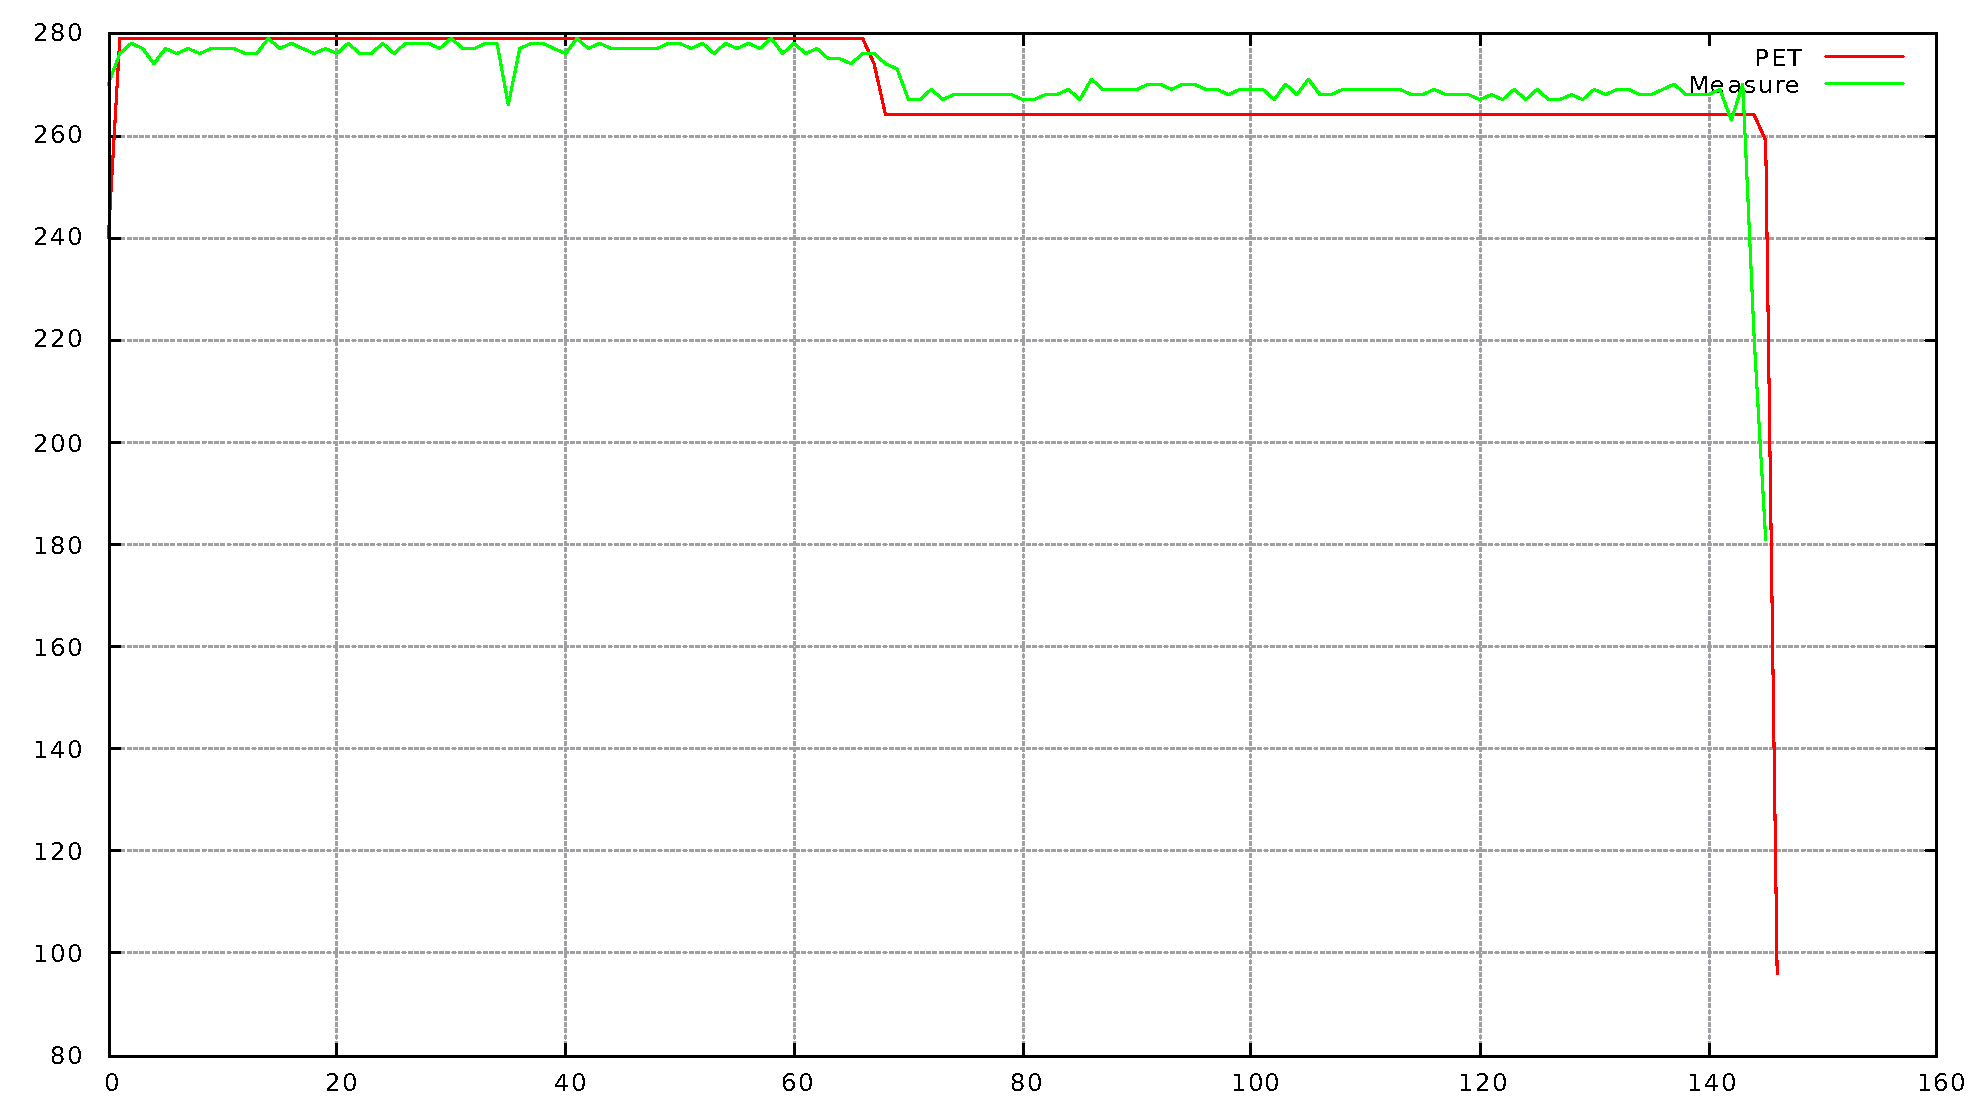
\includegraphics[width=\textwidth]{figs/trend-training.pdf}
\caption{Overlay of PET training results (red) and training data (green)}
\label{fig:trend-training}
\end{figure}


\section{Performance of similar tools}
How good is McPAT, LLVM, other such? (Have not found much, maybe there is a reason for that?)


\section{Conclusion}

PET, Power Estimation Tool, is a software tool for estimating power consumption
on existing as well as non-existing computer architectures.  It uses output from
gem5 together with a set of weighted parameters to estimate energy consumption
of a program on a given hardware model. The weighted parameters are selected by
investigating the pipeline of an ARM Cortex-A9 processor. We have run a set of
workloads on the hardware platform an logged their current drain over time.
Further, the results was used as input for a genetic algorithm that mapped the
correct energy usage to each architectural event in the simulator.

PET is not designed to be as accurate as possible, but to assist hardware
developers as early in the design stage as possible. As opposed to classical
methods, PET can be applied to a design already when only a simulation model
exists. Well known tools such as Wattch or McPAT also utilizes a simulator, but
requires more knowledge about the final hardware, e.g. RTL and process
technology. Irrespective such information, PET is able to estimate current drain
within 10~\% of actual drain when testing against the ARM Cortex-A9 processor.

Because PET is tool meant to be used early and rapidly in the design phase, it
has to be fast and easy to use. PET will predict power usage from log files and
is tested to evaluate 133~MB of log files per second on an Intel Core i7 4820.
Even with log files expanding tens of gigabytes, running PET takes less time
than running a simulator.

An excessive amount of time has been used for tweaking PET, gem5 and the genetic
algorithm to match our reference hardware platform as good as possible. Still,
we believe that the effort needed to port our methods to a new hardware platform
or architecture is much less. The genetic algorithm was in our case able to find
good weights within few hours, and with carefully selected power consuming
events it is likely that this is the same for other architectures. Unrealized
hardware still needs similar hardware to generate data for the weights.

Our observation is that PET allows evaluation of the big picture much easier and
earlier in the design stage than other existing options, simply because it
calculates power with less hardware details. We hope that PET will be useful
when developing both tiles for SHMAC and processors in general.

All in all, using PET or other tools built from the same concept of weighting
architectural events is possible for a set of scenarios. How exact the model is
will depend on the tuning of gem5 and the genetic algorithm used to match
ammeter measurements. The process of settings weights for PET seems cumbersome,
but for most practical settings the most important thing is to have the weights
reasonably proportioned amongst themselves.

%% include here the other chapters

\renewcommand*{\bibname}{References}
\bibliographystyle{unsrt}
\bibliography{main}

%% Uncomment the following if you have any appendix
\appendix
\addtocontents{toc}{%
 \protect\vspace{1em}% 
 \protect\noindent \bfseries \appendixtocname\protect\par
 \protect\vspace{-.5em}%
}
\renewcommand{\chaptername}{\appendixname}
%% include below possible appendices (chapters)
\chapter{TDT4501: Exploring Instruction Level Energy Efficiency}
\label{RH13}
In the pages to follow, the paper from our fall specialization project (TDT4501)
is attached. Raw data and source code used to create that project can be found at github.com
and can be cloned with:
\begin{lstlisting}[language=bash,numbers=none]
git clone https://github.com/terjr/arm-project.git
\end{lstlisting}

\noindent The fall project solved part 1 of the problem as described in the problem description:\hfill\\
\begin{quote}
    \emph{Investigate the power/energy
consumption of simple benchmark programs on real hardware, i.e. create benchmark
programs and evaluate performance by measurements.}
\end{quote}

Hardware and test setup is the same as used in the thesis.

\vfill
\newpage

\thispagestyle{empty}
\hfill
\vfill

\newpage
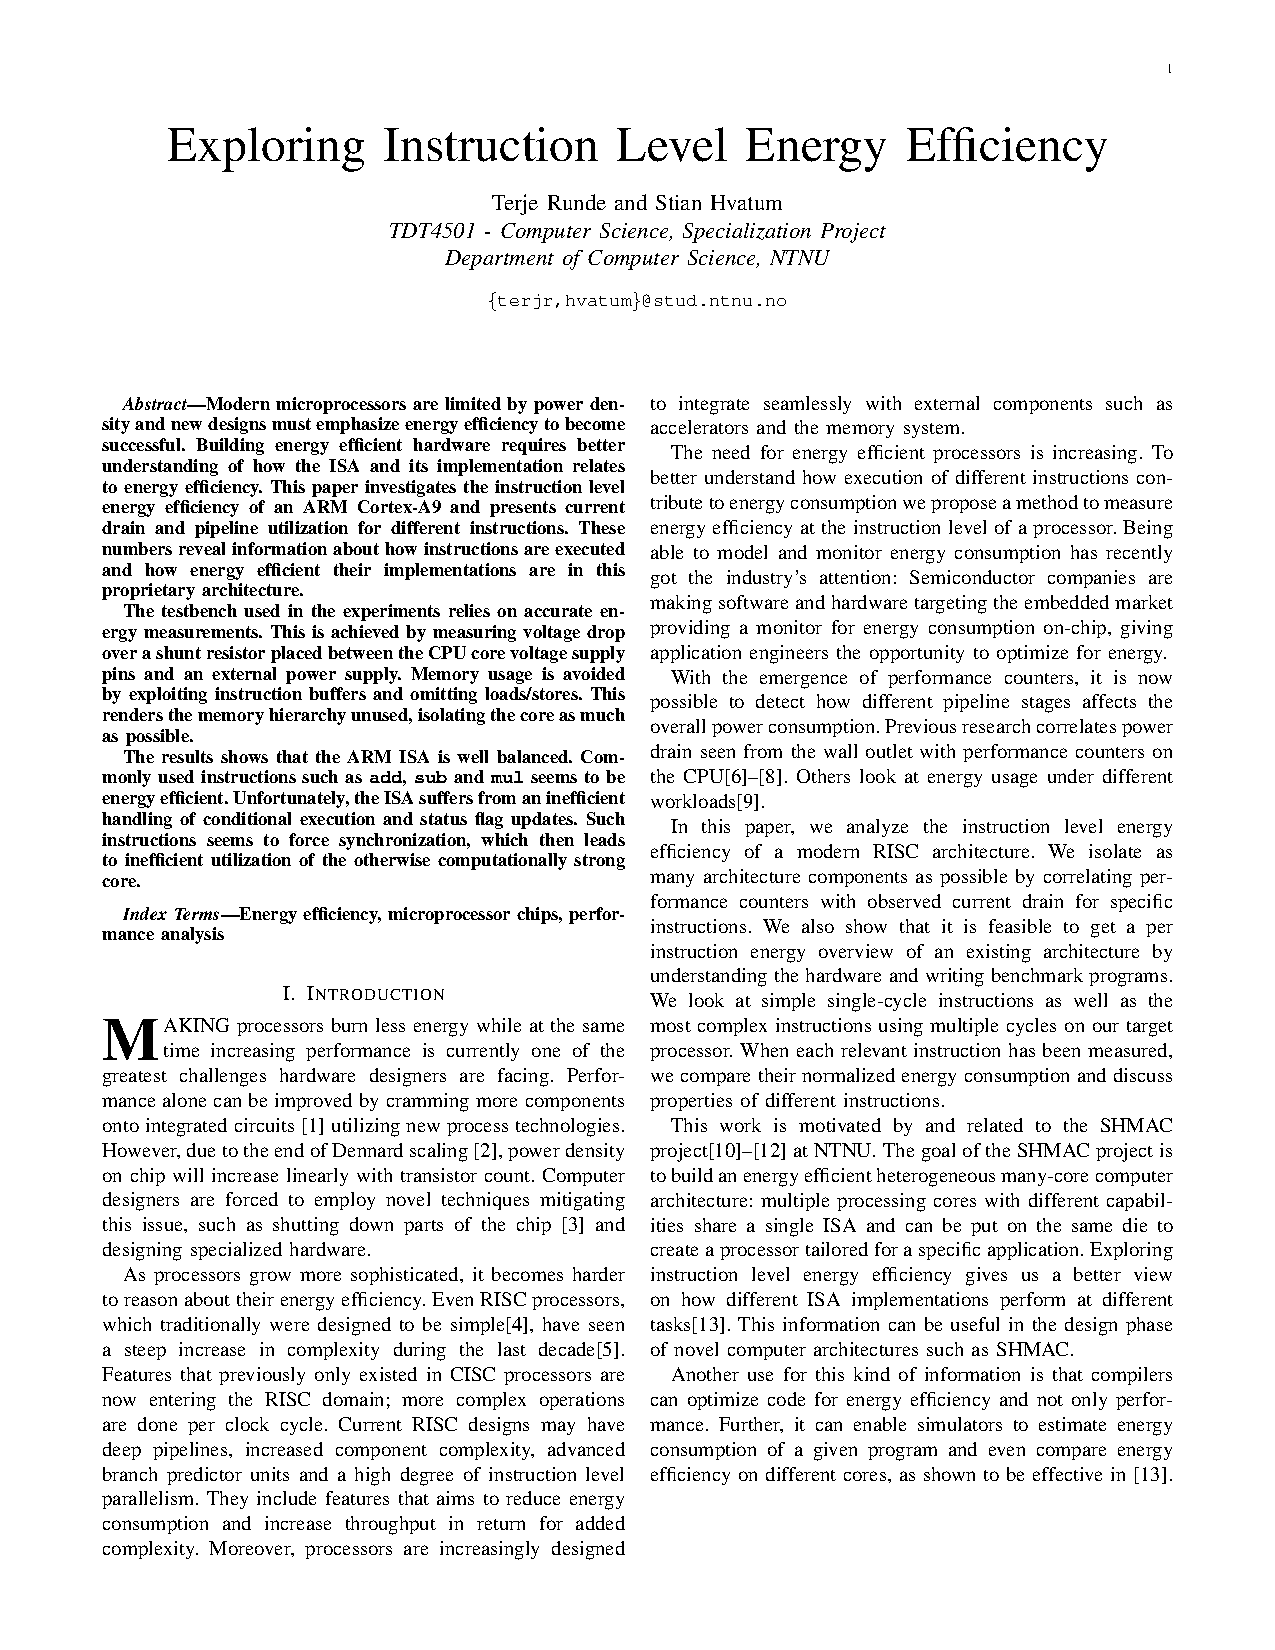
\includepdf[pages=-]{prosjektoppgave.pdf}
\chapter{Modifications to gem5}
\label{apx:gem5files}
All file paths are relative to the root of gem5. Diffs are based of gem5-stable revision aaf017eaad7d.

\section{configs/common/Exynos\_4412P.py}
\label{gem5exynos4412p}
\lstinputlisting[language=python,basicstyle=\tiny,numberstyle=\tiny]{../gem5-configs/Exynos_4412P.py}
\vfill

\section{configs/example/se.py}
\begin{lstlisting}[language=python]
diff --git a/configs/example/se.py b/configs/example/se.py
--- a/configs/example/se.py
+++ b/configs/example/se.py
@@ -104,7 +104,7 @@
         idx += 1
 
     if options.smt:
-        assert(options.cpu_type == "detailed" or options.cpu_type == "inorder")
+        assert(options.cpu_type == "arm_detailed" or options.cpu_type == "inorder")
         return multiprocesses, idx
     else:
         return multiprocesses, 1
@@ -219,7 +219,7 @@
     system.cpu[i].createThreads()
 
 if options.ruby:
-    if not (options.cpu_type == "detailed" or options.cpu_type == "timing"):
+    if not (options.cpu_type == "arm_detailed" or options.cpu_type == "timing"):
         print >> sys.stderr, "Ruby requires TimingSimpleCPU or O3CPU!!"
         sys.exit(1)
 
@@ -255,4 +255,5 @@
     MemConfig.config_mem(options, system)
 
 root = Root(full_system = False, system = system)
+print options
 Simulation.run(options, root, system, FutureClass)
\end{lstlisting}
\vfill

\section{configs/common/CacheConfig.py}
\begin{lstlisting}[language=python]
diff --git a/configs/common/CacheConfig.py b/configs/common/CacheConfig.py
--- a/configs/common/CacheConfig.py
+++ b/configs/common/CacheConfig.py
@@ -55,9 +55,22 @@
 
         dcache_class, icache_class, l2_cache_class = \
             O3_ARM_v7a_DCache, O3_ARM_v7a_ICache, O3_ARM_v7aL2
+    elif options.cpu_type == "exynos_4412p":
+        try:
+            from Exynos_4412P import *
+        except:
+            print "exynos_4412p is unavailable. Did you compile the O3 model?"
+            sys.exit(1)
+
+        dcache_class, icache_class, l2_cache_class = \
+            Exynos_DCache, Exynos_ICache, ExynosL2
+
     else:
         dcache_class, icache_class, l2_cache_class = \
             L1Cache, L1Cache, L2Cache
+    print dcache_class
+    print icache_class
+    print l2_cache_class
 
     # Set the cache line size of the system
     system.cache_line_size = options.cacheline_size
@@ -71,8 +84,9 @@
                                    size=options.l2_size,
                                    assoc=options.l2_assoc)
 
+        print system.cpu_clk_domain
         system.tol2bus = CoherentBus(clk_domain = system.cpu_clk_domain,
-                                     width = 32)
+                                     width = 64)
         system.l2.cpu_side = system.tol2bus.master
         system.l2.mem_side = system.membus.slave
 
\end{lstlisting}
\vfill

\section{configs/common/CpuConfig.py}
\begin{lstlisting}[language=python]
diff --git a/configs/common/CpuConfig.py b/configs/common/CpuConfig.py
--- a/configs/common/CpuConfig.py
+++ b/configs/common/CpuConfig.py
@@ -116,6 +116,13 @@
 except:
     pass
 
+
+try:
+    from Exynos_4412P import Exynos_3
+    _cpu_classes["exynos_4412p"] = Exynos_3
+except:
+    pass
+
 # Add all CPUs in the object hierarchy.
 for name, cls in inspect.getmembers(m5.objects, is_cpu_class):
     _cpu_classes[name] = cls
\end{lstlisting}
\vfill

\section{src/arch/arm/linux/process.cc}
\begin{lstlisting}[language=C++]
diff --git a/src/arch/arm/linux/process.cc b/src/arch/arm/linux/process.cc
--- a/src/arch/arm/linux/process.cc
+++ b/src/arch/arm/linux/process.cc
@@ -66,7 +66,7 @@
 
     strcpy(name->sysname, "Linux");
     strcpy(name->nodename, "m5.eecs.umich.edu");
-    strcpy(name->release, "3.0.0");
+    strcpy(name->release, "3.10.2");
     strcpy(name->version, "#1 Mon Aug 18 11:32:15 EDT 2003");
     strcpy(name->machine, "armv7l");
\end{lstlisting}
\vfill

\section{scr/mem/SimpleDRAM.py}
\label{gem5simpledram}
\begin{lstlisting}[language=python,basicstyle=\tiny,numberstyle=\tiny]
diff --git a/src/mem/SimpleDRAM.py b/src/mem/SimpleDRAM.py
--- a/src/mem/SimpleDRAM.py
+++ b/src/mem/SimpleDRAM.py
@@ -258,6 +258,62 @@
     tXAW = '50ns'
     activation_limit = 4
 
+# A single LPDDR2-S4 x32 400MHz interface (one command/address bus)
+class LPDDR2_S4_800_x32(SimpleDRAM):
+    # 1x32 configuration, 1 device with a 32-bit interface
+    device_bus_width = 32
+
+    # LPDDR2_S4 is a BL4 and BL8 device
+    burst_length = 8
+
+    # Each device has a page (row buffer) size of 1KB
+    # (this depends on the memory density)
+    device_rowbuffer_size = '1kB'
+
+    # 1x32 configuration, so 1 device
+    devices_per_rank = 1
+
+    # Use a single rank
+    ranks_per_channel = 1
+
+    # LPDDR2-S4 has 8 banks in all configurations
+    banks_per_rank = 8
+
+    # Fixed at 15 ns
+    tRCD = '15ns'
+
+    # 8 CK read latency, 4 CK write latency @ 533 MHz, 1.876 ns cycle time
+    tCL = '15ns'
+
+    # Pre-charge one bank 15 ns (all banks 18 ns)
+    tRP = '15ns'
+    tRAS = '42ns'
+
+    # 8 beats across an x32 DDR interface translates to 4 clocks @ 400 MHz.
+    # Note this is a BL8 DDR device.
+    # Requests larger than 32 bytes are broken down into multiple requests
+    # in the controller
+    tBURST = '7.5ns'
+
+    # LPDDR2-S4, 16Gbit
+    tRFC = '210ns'
+    tREFI = '3.9us'
+
+    # Irrespective of speed grade, tWTR is 7.5 ns
+    tWTR = '7.5ns'
+
+    # Activate to activate irrespective of density and speed grade
+    tRRD = '10.0ns'
+
+    # Irrespective of density, tFAW is 50 ns
+    tXAW = '50ns'
+    activation_limit = 4
+
 # A single WideIO x128 interface (one command and address bus), with
 # default timings based on an estimated WIO-200 8 Gbit part.
 class WideIO_200_x128(SimpleDRAM):
\end{lstlisting}
\vfill



\newpage
\thispagestyle{empty}
\vfill
\newpage
\thispagestyle{empty}
\centering
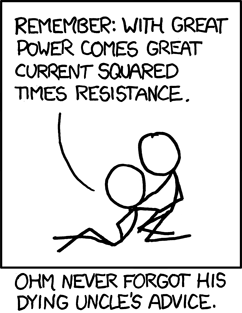
\includegraphics{figs/ohm.png}
\vfill

\end{document} 
